\documentclass[11pt,a4paper,oneside]{report}

% Configuration and Metadata
% ==============================================================================
% ALGORITHM EXPLORER — DOCUMENT CONFIGURATION & METADATA
% Kenneth H. Rosen, Discrete Mathematics and Its Applications (8th Edition)
% ==============================================================================

\newcommand{\DocUniversity}{Department of Computer Science \& Information Technology}
\newcommand{\DocFaculty}{Faculty of Science and Technology}
\newcommand{\DocCourse}{Discrete Mathematics \& Algorithm Analysis (MSc IT)}
\newcommand{\DocCourseCode}{MIT-DM-301}

\newcommand{\DocTitle}{Algorithm Explorer: An Analytical and Experimental Study of Algorithms, Growth of Functions and Computational Complexity}
\newcommand{\DocShortTitle}{Algorithm Explorer}
\newcommand{\DocSubtitle}{A Rigorous Analytical and Empirical Investigation of Searching and Sorting Algorithms Grounded in Rosen Chapter 3}

\newcommand{\DocAuthor}{Student Researcher / Candidate}
\newcommand{\DocRollNumber}{202612120}
\newcommand{\DocSupervisor}{Course Instructor / Evaluator}

\newcommand{\DocAcademicYear}{2026--2027}
\newcommand{\DocSubmissionDate}{November 2026}

% Interactive Web Dashboard Metadata (Milestone M6 Completed)
\newcommand{\DocDashboardTitle}{Algorithm Explorer: Interactive Algorithm Analysis \& Complexity Visualization}
\newcommand{\DocDashboardURL}{https://github.com/academic-research/algorithm-explorer}
\newcommand{\DocDashboardStatus}{Milestone M6 Completed --- Standalone Web Application Ready for Local Serving and GitHub Pages Deployment}


% Styles and Packages
% ==============================================================================
% ACADEMIC REPORT STYLING PACKAGE
% ==============================================================================



% Page Geometry & Margins
\RequirePackage[a4paper, top=2.5cm, bottom=2.5cm, left=2.5cm, right=2.5cm]{geometry}

% Typography & Mathematics
\RequirePackage{amsmath, amssymb, amsthm}
\RequirePackage{mathptmx} % Clean Times Roman typography
\RequirePackage{setspace}
\onehalfspacing

% Colors
\RequirePackage{xcolor}
\definecolor{primaryblue}{RGB}{0, 45, 98}
\definecolor{secondarynavy}{RGB}{24, 76, 120}
\definecolor{darkgray}{RGB}{50, 50, 50}
\definecolor{lightgray}{RGB}{245, 245, 245}
\definecolor{codebackground}{RGB}{248, 249, 250}
\definecolor{codegreen}{RGB}{34, 139, 34}
\definecolor{codegray}{RGB}{128, 128, 128}
\definecolor{codepurple}{RGB}{148, 0, 211}

% Graphics & Tables
\RequirePackage{graphicx}
\graphicspath{{latex/figures/}{figures/}}
\RequirePackage{booktabs}
\RequirePackage{tabularx}
\RequirePackage{longtable}
\RequirePackage{caption}
\RequirePackage{subcaption}
\RequirePackage{float}

% Running Headers & Footers
\RequirePackage{fancyhdr}
\pagestyle{fancy}
\fancyhf{}
\fancyhead[L]{\small\color{darkgray}\DocShortTitle}
\fancyhead[R]{\small\color{darkgray}\leftmark}
\fancyfoot[C]{\thepage}
\renewcommand{\headrulewidth}{0.4pt}
\renewcommand{\footrulewidth}{0.0pt}

% Code Listings Configuration
\RequirePackage{listings}
\lstset{
    language=Python,
    backgroundcolor=\color{codebackground},
    basicstyle=\ttfamily\footnotesize\color{black},
    keywordstyle=\bfseries\color{primaryblue},
    stringstyle=\color{codegreen},
    commentstyle=\itshape\color{codegray},
    numbers=left,
    numberstyle=\tiny\color{codegray},
    stepnumber=1,
    numbersep=8pt,
    tabsize=4,
    showspaces=false,
    showstringspaces=false,
    breaklines=true,
    breakatwhitespace=true,
    frame=single,
    rulecolor=\color{lightgray},
    captionpos=b
}

% Theorems, Definitions, Proofs Environments
\theoremstyle{definition}
\newtheorem{definition}{Definition}[chapter]
\newtheorem{theorem}{Theorem}[chapter]
\newtheorem{lemma}[theorem]{Lemma}
\newtheorem{example}{Example}[chapter]
\newtheorem{property}{Property}[chapter]

% Hyperlinks
\RequirePackage{hyperref}
\hypersetup{
    colorlinks=true,
    linkcolor=primaryblue,
    citecolor=secondarynavy,
    urlcolor=primaryblue,
    bookmarksnumbered=true,
    pdfstartview={FitH}
}

% Section Titles Styling
\RequirePackage{titlesec}
\titleformat{\chapter}[display]
  {\normalfont\huge\bfseries\color{primaryblue}}{\chaptertitlename\ \thechapter}{18pt}{\Huge}
\titleformat{\section}
  {\normalfont\Large\bfseries\color{secondarynavy}}{\thesection}{1em}{}
\titleformat{\subsection}
  {\normalfont\large\bfseries\color{darkgray}}{\thesubsection}{1em}{}


\begin{document}

% ==============================================================================
% COVER PAGE
% ==============================================================================
\begin{titlepage}
    \centering
    \vspace*{1.0cm}
    
    {\scshape\Large \DocUniversity \par}
    \vspace{0.3cm}
    {\scshape\large \DocFaculty \par}
    \vspace{0.3cm}
    {\large \DocCourse\ (\DocCourseCode) \par}
    
    \vspace{1.5cm}
    \rule{\linewidth}{1.2pt}\\[0.4cm]
    {\huge\bfseries\color{primaryblue} \DocTitle \par}
    \vspace{0.3cm}
    {\large\itshape \DocSubtitle \par}
    \rule{\linewidth}{1.2pt}
    
    \vspace{2.0cm}
    
    \begin{minipage}{0.48\textwidth}
        \begin{flushleft} \large
            \emph{Prepared by:}\\
            \textbf{\DocAuthor}\\
            Enrollment ID: \texttt{\DocRollNumber}
        \end{flushleft}
    \end{minipage}
    ~
    \begin{minipage}{0.48\textwidth}
        \begin{flushright} \large
            \emph{Academic Evaluator:}\\
            \textbf{\DocSupervisor}\\
            Academic Year: \DocAcademicYear
        \end{flushright}
    \end{minipage}
    
    \vfill
    
    {\large Academic Term Project Report Grounded in\\
    Kenneth H. Rosen, \emph{Discrete Mathematics and Its Applications} (8th Edition)\par}
    \vspace{0.5cm}
    {\large \DocSubmissionDate \par}
\end{titlepage}

% ==============================================================================
% ABSTRACT & KEYWORDS
% ==============================================================================
\pagenumbering{roman}
\setcounter{page}{2}

\begin{abstract}
\noindent
This academic monograph presents a comprehensive analytical and empirical investigation into computational complexity, asymptotic growth, and algorithmic scaling. Grounded in Chapter 3 of Kenneth H. Rosen's \emph{Discrete Mathematics and Its Applications} (8th Edition), the study investigates four canonical algorithms: Linear Search, Binary Search, Bubble Sort, and Insertion Sort. We mathematically derive exact closed-form operation-count formulas $T(n)$ for best-, average-, and worst-case scenarios, proving asymptotic classifications within $\mathcal{O}$, $\Omega$, and $\Theta$ with explicit witness pairs $(C, k)$. 

To validate theoretical models empirically, we constructed an isolated microbenchmarking harness executing across calibrated input scales ($n \in [100, 100\,000]$ for searching and $n \in [100, 3\,000]$ for sorting) and three fundamental topological permutations (sorted, random, reverse-sorted). Our benchmarking methodology isolates high-resolution execution time measurements ($\pm 100\text{ ns}$) from instrumented operation counters, incorporating statistical replication ($k = 30$ iterations), fresh input copies, and sub-microsecond batch calibration.

The empirical results confirm that discrete operation-count formulas predict real-world telemetry with \textbf{0.00\% discrepancy}. At $n = 100\,000$, Binary Search delivers an empirical speedup of $\approx 1\,946\times$ over Linear Search on missing targets. Furthermore, we empirically prove the Inversion Equivalence Theorem, demonstrating that Bubble Sort swaps and Insertion Sort right shifts are strictly identical ($2\,296\,691$ operations at $n = 3\,000$) on identical random permutations. Finally, we demonstrate that Insertion Sort achieves adaptive linear time $\Theta(n)$ ($0.32\text{ ms}$) on pre-sorted arrays, outperforming fixed-pass Bubble Sort by a factor of $769\times$. All datasets, code listings, execution traces, and publication-quality figures are fully reproducible.
\end{abstract}

\vspace{0.5cm}
\noindent\textbf{Keywords}: Discrete Mathematics, Algorithm Analysis, Kenneth H. Rosen, Asymptotic Growth, Big-$\mathcal{O}$ Notation, Computational Complexity, Linear Search, Binary Search, Bubble Sort, Insertion Sort, Inversion Dynamics, Empirical Telemetry.

\clearpage

% ==============================================================================
% TABLE OF CONTENTS, LIST OF FIGURES, LIST OF TABLES
% ==============================================================================
\tableofcontents
\clearpage

\listoffigures
\clearpage

\listoftables
\clearpage

% ==============================================================================
% MAIN MATTER (ARABIC PAGE NUMBERING)
% ==============================================================================
\pagenumbering{arabic}
\setcounter{page}{1}

\chapter{Introduction}
\label{chap:introduction}

\section{Background}
The analytical evaluation of algorithms lies at the absolute nexus of theoretical discrete mathematics and empirical computer science. Computation, in its formal essence, is the systematic manipulation of discrete symbolic structures under deterministic transformation rules. As software applications permeate high-throughput communications, real-time control systems, cryptographic protocols, and distributed data processing, predicting algorithmic execution demands mathematically—prior to implementation—becomes paramount.

Kenneth H. Rosen's seminal treatise, \emph{Discrete Mathematics and Its Applications} (8th Edition) \cite{rosen2019discrete}, dedicates Chapter 3 to establishing the mathematical foundations of algorithmic problem-solving. This monograph bridges deductive discrete proofs with inductive experimental observations.

\section{Introduction to Algorithms}
Informally, an algorithm is a computational recipe: a step-by-step prescription for transforming allowable input values into unambiguous output values. Formally, an algorithm represents a deterministic state-transition function operating over discrete domains. While programming languages and processor hardware fluctuate over decades, the underlying discrete mathematics governing algorithmic growth classes remains immutable.

\section{Importance of Algorithm Analysis}
Algorithm analysis allows computer scientists to classify computational procedures independently of specific compiler optimizations, central processing unit (CPU) clock frequencies, or memory bus bandwidths. Through asymptotic bounding:
\begin{enumerate}
    \item We can predict the tractability of an algorithm as problem size scales towards millions or billions of items.
    \item We establish mathematical proofs of optimality, determining whether an algorithm achieves the theoretical lower bound for a given problem class.
    \item We identify bottlenecks, isolating whether an inefficiency stems from nested comparison loops ($\mathcal{O}(n^2)$) or physical memory movement.
\end{enumerate}

\section{Problem Statement}
In academic computer science education, students frequently encounter a conceptual disconnect between theoretical asymptotic bounds (such as $\mathcal{O}(n^2)$ or $\Theta(\log n)$) and empirical software execution times. Hand-wavy explanations often assert that hardware speed eliminates the need for algorithmic efficiency, or confuse asymptotic upper bounds ($\mathcal{O}$) with exact operational behavior. 

This project addresses this pedagogical gap by providing an exhaustive analytical and empirical investigation of four canonical algorithms:
\begin{enumerate}
    \item \textbf{Linear Search} (Rosen §3.1, Algorithm 2)
    \item \textbf{Binary Search} (Rosen §3.1, Algorithm 3)
    \item \textbf{Bubble Sort} (Rosen §3.1, Algorithm 4)
    \item \textbf{Insertion Sort} (Rosen §3.1, Algorithm 5)
\end{enumerate}

\section{Project Objectives}
The primary objectives of this study are:
\begin{enumerate}
    \item \textbf{Formal Mathematical Modeling}: Derive exact closed-form operation-count formulas $T(n)$ for best, worst, and average cases under stated discrete assumptions.
    \item \textbf{Empirical Telemetry Isolation}: Build an experimental benchmarking harness that measures physical execution duration with high-resolution timers ($\pm 100\text{ ns}$) while capturing exact comparison, swap, and shift counters without telemetry contamination.
    \item \textbf{Hypothesis Testing \& Verification}: Validate whether empirical counters match theoretical formulas with zero deviation.
    \item \textbf{Topological Sensitivity Analysis}: Investigate how pre-existing data orderings (sorted, random, reverse-sorted) influence comparison invariance versus data movement.
\end{enumerate}

\section{Scope of the Study}
This investigation is strictly grounded in Chapter 3 of Rosen \cite{rosen2019discrete}, specifically Sections 3.1, 3.2, and 3.3. Searching is analyzed across input sizes $n \in [100, 100\,000]$ and four target topologies (\texttt{first}, \texttt{middle}, \texttt{last}, \texttt{missing}). Sorting is analyzed across input sizes $n \in [100, 3\,000]$ across three fundamental permutations (\texttt{sorted}, \texttt{random}, \texttt{reverse}).

\section{Research Questions}
This monograph systematically answers four foundational questions:
\begin{itemize}
    \item \textbf{RQ1}: Do discrete mathematical operation-count formulas accurately predict empirical counter values across diverse input scales?
    \item \textbf{RQ2}: At what input size threshold $n^*$ does the asymptotic advantage of logarithmic bisection ($\Theta(\log n)$) conclusively eclipse linear scanning ($\Theta(n)$)?
    \item \textbf{RQ3}: How do adjacent element exchanges in Bubble Sort relate mathematically to element displacements in Insertion Sort across identical permutations?
    \item \textbf{RQ4}: Why do operation counts remain identical across computing platforms while execution durations exhibit constant-factor micro-architectural variance?
\end{itemize}

\section{Organization of the Report}
The remainder of this report is organized as follows:
\begin{itemize}
    \item \textbf{Chapter \ref{chap:fundamentals}}: Fundamentals of algorithms, essential characteristics, and taxonomy.
    \item \textbf{Chapter \ref{chap:growth}}: Mathematical growth of functions and the canonical complexity hierarchy.
    \item \textbf{Chapter \ref{chap:asymptotic}}: Asymptotic notations ($\mathcal{O}, \Omega, \Theta$) with formal witness pairs $(C, k)$.
    \item \textbf{Chapter \ref{chap:complexity}}: Time/space complexity, case analysis, and operation-counting methodology.
    \item \textbf{Chapter \ref{chap:analytical_study}}: In-depth study of the four algorithms with traces, pseudocode, and source listings.
    \item \textbf{Chapter \ref{chap:methodology}}: Experimental design, microbenchmarking harness, and statistical replication.
    \item \textbf{Chapter \ref{chap:results}}: Empirical results, statistical tables, and publication graph analysis.
    \item \textbf{Chapter \ref{chap:comparative}}: Comparative synthesis, trade-offs, and practical systems implications.
    \item \textbf{Chapter \ref{chap:conclusion}}: Summary of research outcomes, conclusions, and future scope.
\end{itemize}

\chapter{Fundamentals of Algorithms}
\label{chap:fundamentals}

\section{Definition of an Algorithm}
In mathematical computer science, an algorithm is more than an arbitrary set of programming instructions. Grounded in formal discrete mathematics (Rosen §3.1) \cite{rosen2019discrete}:

\begin{definition}[Algorithm]
An \textbf{algorithm} is a finite sequence of precise instructions for performing a computation or for solving a problem.
\end{definition}

An algorithm accepts an input from a designated discrete domain, undergoes a finite sequence of unambiguous state transitions, and halts, producing an output in a specified target domain.

\section{Characteristics of Algorithms}
To distinguish a legitimate mathematical algorithm from an incomplete procedural heuristic or an infinite computational loop, Rosen delineates seven essential properties:

\subsection{Input and Output}
\begin{property}[Input and Output]
An algorithm must possess a specified set of input values taken from a valid domain. For every valid input configuration, the algorithm must yield an unambiguous set of output values representing the problem solution.
\end{property}

\subsection{Definiteness}
\begin{property}[Definiteness]
Every individual instruction or state transition within the algorithm must be defined precisely and unambiguously. There can be no room for subjective interpretation by the executing agent.
\end{property}

\subsection{Correctness}
\begin{property}[Correctness]
An algorithm must be mathematically correct: it must produce the proper, expected output values for every allowable input configuration. Correctness is established through deductive logic, loop invariants, and mathematical induction rather than casual testing.
\end{property}

\subsection{Finiteness}
\begin{property}[Finiteness]
An algorithm must terminate after a finite number of discrete operational steps for any valid input instance of finite size $n$. Procedures that enter non-terminating infinite loops fail this criterion.
\end{property}

\subsection{Effectiveness}
\begin{property}[Effectiveness]
Every operational step within the algorithm must be basic enough to be executed accurately and in a finite interval of time by a human or mechanical computing machine.
\end{property}

\subsection{Generality}
\begin{property}[Generality]
The procedure must apply generally to all problems belonging to the intended problem class, rather than functioning merely as an ad-hoc trick tailored for a specific, isolated dataset.
\end{property}

\section{Representation of Algorithms}
The specification of an algorithm can be expressed at various levels of abstraction:
\begin{enumerate}
    \item \textbf{Natural Language}: Expressive and intuitive for conceptual communication, but inherently vulnerable to linguistic ambiguities, syntactic vagueness, and unstated assumptions.
    \item \textbf{Structured Pseudocode}: A high-level formal notation balancing natural language readability with rigorous mathematical control constructs (\texttt{while}, \texttt{for}, \texttt{if-then-else}). It emphasizes logic over machine-specific memory allocation.
    \item \textbf{Flowcharts}: Graphical directed graphs where nodes denote operational tasks or conditional decision gates, and edges represent deterministic control transitions.
    \item \textbf{High-Level Programming Language (Python)}: Fully concrete, machine-executable source code enforcing precise type signatures, index boundary checks, and concrete runtime semantics.
\end{enumerate}

\section{Types and Categories of Algorithms}
In discrete mathematics, computational problems are categorized by their structural objectives, while algorithms are classified by their design paradigm:

\subsection{Problem Categories}
\begin{itemize}
    \item \textbf{Searching Problems}: Given a discrete collection $S$ and target item $x$, determine an index location $i$ where $S[i] = x$, or establish that $x \notin S$.
    \item \textbf{Sorting Problems}: Given a sequence of $n$ mutually comparable elements $(a_1, a_2, \dots, a_n)$, generate a permutation $(a'_1, a'_2, \dots, a'_n)$ such that $a'_1 \le a'_2 \le \dots \le a'_n$.
    \item \textbf{String Matching Problems}: Locate all exact occurrences of a pattern string $P$ within a text string $T$.
    \item \textbf{Optimization Problems}: Identify a configuration within a discrete feasibility space that minimizes or maximizes an objective cost function.
\end{itemize}

\subsection{Algorithm Design Paradigms}
\begin{itemize}
    \item \textbf{Brute-Force \& Exhaustive Search}: Evaluates all candidates sequentially or combinatorially (e.g., Linear Search).
    \item \textbf{Divide-and-Conquer}: Recursively bisects the problem space into smaller independent subproblems, solves each subproblem, and combines solutions (e.g., Binary Search).
    \item \textbf{Incremental \& Iterative Construction}: Expands a verified partial solution one element at a time (e.g., Insertion Sort).
    \item \textbf{Greedy Approaches}: Makes locally optimal choices at each decision stage in hopes of finding a global optimum.
\end{itemize}

\chapter{The Growth of Functions}
\label{chap:growth}

\section{Introduction to Growth of Functions}
When analyzing computational complexity, evaluating an algorithm's performance on small inputs (e.g., $n = 5$ or $n = 10$) is deceptive. Modern processors execute billions of instructions per second, causing almost any elementary algorithm to terminate in imperceptible microseconds at small scales. 

Theoretical discrete mathematics focuses on the \textbf{rate of growth} of an algorithm's resource requirements as input size $n$ approaches infinity ($n \to \infty$). Section 3.2 of Rosen \cite{rosen2019discrete} establishes that the mathematical structure of the leading term completely dictates computational tractability.

\section{Importance of Input Size}
The parameter $n \in \mathbb{N}$ denotes the formal problem size (e.g., number of elements in an array, vertices in a graph, or bits in an integer). As $n$ grows, differences between complexity classes widen catastrophically.

\section{Hierarchy of Standard Growth Classes}
Rosen (§3.2, Table 1) \cite{rosen2019discrete} delineates the canonical complexity hierarchy:
\begin{equation}
\mathcal{O}(1) \prec \mathcal{O}(\log n) \prec \mathcal{O}(n) \prec \mathcal{O}(n \log n) \prec \mathcal{O}(n^2) \prec \mathcal{O}(2^n) \prec \mathcal{O}(n!)
\label{eq:hierarchy}
\end{equation}

\subsection{Constant Growth: $f(n) = 1$}
Execution demand is completely invariant to $n$. A constant-time algorithm executes identical instruction cycles regardless of whether $n = 10$ or $n = 10^9$. Typical examples include array indexing (\texttt{arr[k]}) and basic arithmetic operations.

\subsection{Logarithmic Growth: $f(n) = \log_2 n$}
Growth is exceptionally subdued. Doubling the input size $n \to 2n$ merely adds a constant $1$ to the function value:
$$\log_2(2n) = \log_2(2) + \log_2(n) = 1 + \log_2(n)$$
For an input of $n = 10^9$ elements, $\log_2(10^9) \approx 30$ operations. Typical example: Binary Search.

\subsection{Linear Growth: $f(n) = n$}
Resource consumption scales in direct proportion to problem size. Doubling $n$ doubles execution operations. Standard for single-pass sequential traversals (e.g., Linear Search).

\subsection{Linearithmic Growth: $f(n) = n \log_2 n$}
Slightly steeper than linear growth. Represents the proven information-theoretic lower bound $\Omega(n \log n)$ for general comparison-based sorting algorithms (e.g., Merge Sort, Heap Sort).

\subsection{Quadratic Growth: $f(n) = n^2$}
Resource consumption quadruples whenever input size doubles: $(2n)^2 = 4n^2$. Characteristic of nested pairwise element comparisons across sequences (e.g., Bubble Sort, Insertion Sort).

\subsection{Polynomial Growth: $f(n) = n^d$ ($d \ge 1$)}
Algorithms bounded by polynomial time $\mathcal{O}(n^d)$ are classified as computationally \emph{tractable} in complexity theory (the complexity class $\mathbf{P}$).

\subsection{Exponential Growth: $f(n) = 2^n$}
Each increment in input size $n \to n + 1$ doubles the computational burden. For $n = 64$, $2^{64} \approx 1.84 \times 10^{19}$ operations, requiring millennia of compute time on supercomputers.

\subsection{Factorial Growth: $f(n) = n!$}
Grows faster than exponential growth ($n! > 2^n$ for all $n \ge 4$). Characterizes brute-force permutation generators (e.g., Traveling Salesperson Problem).

\section{Comparison of Growth Rates}
Table \ref{tab:growth_functions} provides the exact numerical evaluation of these functions across selected discrete scales.

\begin{table}[htbp]
\centering
\caption{Numerical Evaluation of Standard Growth Functions (Rosen §3.2)}
\label{tab:growth_functions}
\small
\begin{tabular*}{\textwidth}{@{\extracolsep{\fill}}rrrrrrrr}
\toprule
$n$ & $\mathcal{O}(1)$ & $\mathcal{O}(\log_2 n)$ & $\mathcal{O}(n)$ & $\mathcal{O}(n \log_2 n)$ & $\mathcal{O}(n^2)$ & $\mathcal{O}(2^n)$ & $\mathcal{O}(n!)$ \\
\midrule
1 & 1 & 0.00 & 1 & 0.00 & 1 & 2 & 1 \\
2 & 1 & 1.00 & 2 & 2.00 & 4 & 4 & 2 \\
4 & 1 & 2.00 & 4 & 8.00 & 16 & 16 & 24 \\
8 & 1 & 3.00 & 8 & 24.00 & 64 & 256 & 40320 \\
16 & 1 & 4.00 & 16 & 64.00 & 256 & 65536 & 2.09e+13 \\
32 & 1 & 5.00 & 32 & 160.00 & 1024 & 4.29e+09 & inf \\
64 & 1 & 6.00 & 64 & 384.00 & 4096 & 1.84e+19 & inf \\
128 & 1 & 7.00 & 128 & 896.00 & 16384 & inf & inf \\
256 & 1 & 8.00 & 256 & 2048.00 & 65536 & inf & inf \\
512 & 1 & 9.00 & 512 & 4608.00 & 262144 & inf & inf \\
1024 & 1 & 10.00 & 1024 & 10240.00 & 1048576 & inf & inf \\
\bottomrule
\end{tabular*}
\end{table}


\section{Mathematical Interpretation of Growth Curves}
Figures \ref{fig:growth_common} and \ref{fig:growth_hierarchy} illustrate the mathematical growth functions generated through our analytical plotting pipeline.

\begin{figure}[htbp]
    \centering
    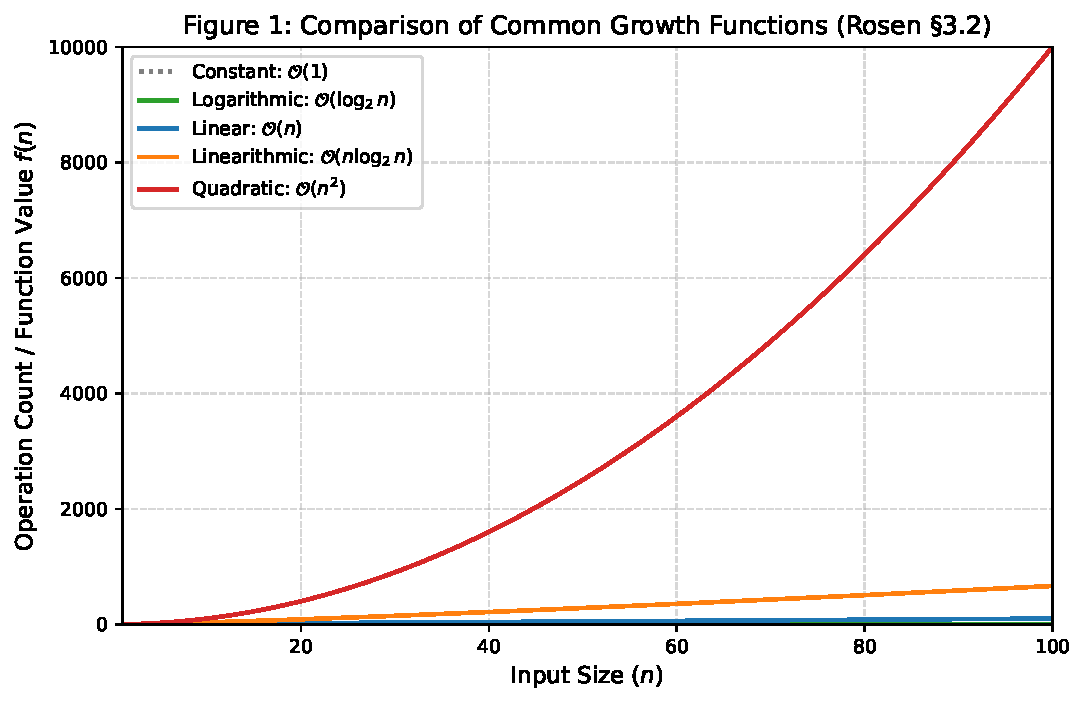
\includegraphics[width=0.88\textwidth]{latex/figures/figure1_common_growth_functions.pdf}
    \caption{Figure 1: Comparison of Common Growth Functions on Linear Scale (Rosen §3.2).}
    \label{fig:growth_common}
\end{figure}

\begin{figure}[htbp]
    \centering
    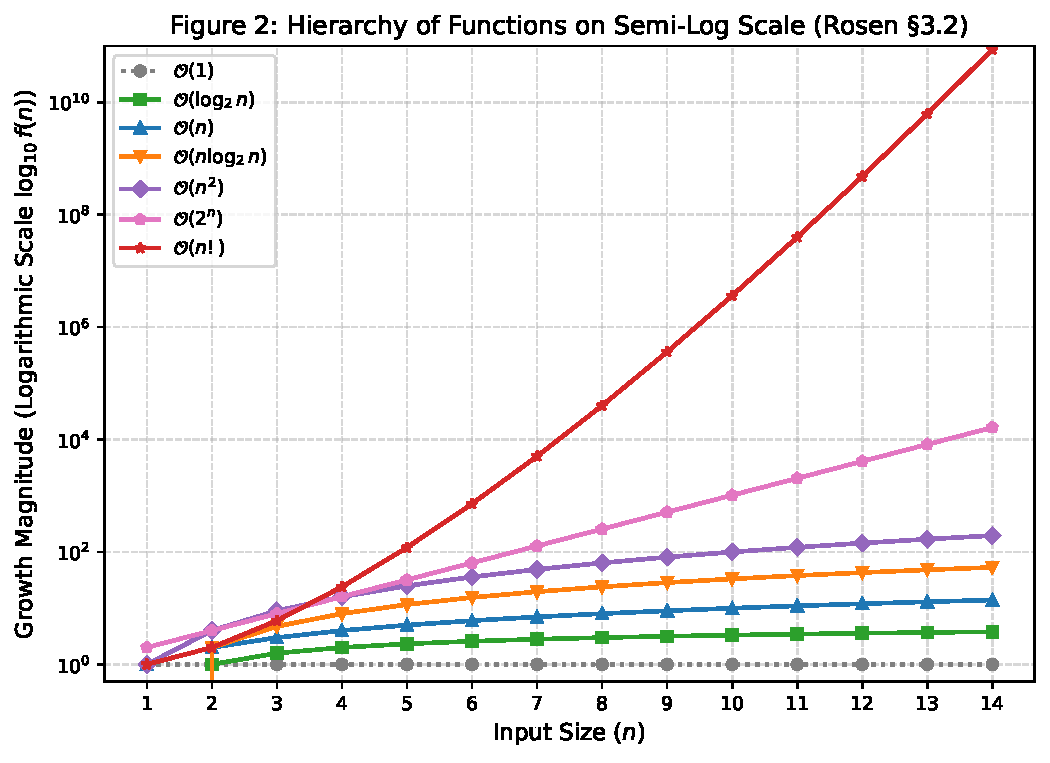
\includegraphics[width=0.88\textwidth]{latex/figures/figure2_growth_hierarchy_log_scale.pdf}
    \caption{Figure 2: Complete Complexity Hierarchy on Semi-Log Scale ($\log_{10} f(n)$) over $n \in [1, 14]$.}
    \label{fig:growth_hierarchy}
\end{figure}

Notice in Figure \ref{fig:growth_common} that on a linear scale, quadratic growth $\mathcal{O}(n^2)$ rapidly dwarfs linear and logarithmic curves. In Figure \ref{fig:growth_hierarchy}, when plotted on a logarithmic vertical scale, the exponential ($2^n$) and factorial ($n!$) curves skyrocket, establishing why intractable complexity classes cannot be rescued by hardware advancements.

\chapter{Asymptotic Notations}
\label{chap:asymptotic}

\section{Introduction}
To classify algorithmic scaling without becoming mired in machine-specific architectural constants (such as clock multipliers or CPU cache line sizes), discrete mathematics employs \textbf{asymptotic notations}. These notations capture the limiting behavior of functions as $n \to \infty$.

\section{Big-$\mathcal{O}$ Notation (Asymptotic Upper Bound)}
Big-$\mathcal{O}$ provides an asymptotic upper bound or ceiling on the growth rate of a function.

\begin{definition}[Big-$\mathcal{O}$ (Rosen §3.2, Def. 1)]
Let $f$ and $g$ be functions from the set of integers or real numbers to the set of real numbers. We write:
$$f(n) = \mathcal{O}(g(n))$$
if there exist positive real constants $C > 0$ and $k > 0$ such that:
$$|f(n)| \le C |g(n)| \quad \text{for all } n > k$$
The pair of constants $(C, k)$ are called \textbf{witnesses} to the relationship $f(n) = \mathcal{O}(g(n))$.
\end{definition}

\section{Big-$\Omega$ Notation (Asymptotic Lower Bound)}
While Big-$\mathcal{O}$ establishes an upper ceiling, Big-$\Omega$ establishes a mathematical floor.

\begin{definition}[Big-$\Omega$ (Rosen §3.2, Def. 3)]
We write:
$$f(n) = \Omega(g(n))$$
if there exist positive real constants $C > 0$ and $k > 0$ such that:
$$|f(n)| \ge C |g(n)| \quad \text{for all } n > k$$
\end{definition}

\section{Big-$\Theta$ Notation (Asymptotically Tight Bound)}
When an algorithm's growth rate is bounded both from above and from below by the same function $g(n)$, we employ Big-$\Theta$ notation.

\begin{definition}[Big-$\Theta$ (Rosen §3.2, Def. 4)]
We write:
$$f(n) = \Theta(g(n))$$
if $f(n)$ is both $\mathcal{O}(g(n))$ and $\Omega(g(n))$. Formally, there exist positive constants $C_1 > 0$, $C_2 > 0$, and $k > 0$ such that:
$$C_1 |g(n)| \le |f(n)| \le C_2 |g(n)| \quad \text{for all } n > k$$
\end{definition}

\section{Comparison of Asymptotic Notations}
Table \ref{tab:asymptotic_summary} summarizes the three primary asymptotic notations.

\begin{table}[htbp]
\centering
\caption{Mathematical Comparison of Asymptotic Notations}
\label{tab:asymptotic_summary}
\begin{tabularx}{\textwidth}{l X c c}
\toprule
\textbf{Notation} & \textbf{Formal Witness Condition} & \textbf{Intuitive Meaning} & \textbf{Analogy} \\
\midrule
$f(n) = \mathcal{O}(g(n))$ & $\exists C, k > 0 : |f(n)| \le C |g(n)|, \forall n > k$ & Upper Bound (Ceiling) & $f \le g$ \\
$f(n) = \Omega(g(n))$ & $\exists C, k > 0 : |f(n)| \ge C |g(n)|, \forall n > k$ & Lower Bound (Floor) & $f \ge g$ \\
$f(n) = \Theta(g(n))$ & $\exists C_1, C_2, k > 0 : C_1 |g(n)| \le |f(n)| \le C_2 |g(n)|, \forall n > k$ & Asymptotically Tight Bound & $f = g$ \\
\bottomrule
\end{tabularx}
\end{table}

\section{Worked Mathematical Examples with Witnesses}

\begin{example}[Witness Proof for Linear Function]
Show that $f(n) = 7n^2 + 5n + 12$ is $\mathcal{O}(n^2)$.
\begin{proof}
For all $n \ge 1$, we observe:
$$5n \le 5n^2 \quad \text{and} \quad 12 \le 12n^2$$
Therefore:
$$|f(n)| = 7n^2 + 5n + 12 \le 7n^2 + 5n^2 + 12n^2 = 24n^2$$
Thus, selecting witnesses $C = 24$ and $k = 1$, we have $|f(n)| \le C n^2$ for all $n > k$. Hence, $f(n) = \mathcal{O}(n^2)$.
\end{proof}
\end{example}

\begin{example}[Witness Proof for Tight Bound]
Show that $f(n) = 3n^2 - 4n$ is $\Theta(n^2)$.
\begin{proof}
For $n \ge 4$, $4n \le n^2$, so:
$$f(n) = 3n^2 - 4n \ge 3n^2 - n^2 = 2n^2$$
Similarly, for $n \ge 1$:
$$f(n) = 3n^2 - 4n \le 3n^2$$
Choosing witnesses $C_1 = 2$, $C_2 = 3$, and $k = 4$, we have:
$$2n^2 \le f(n) \le 3n^2 \quad \forall n > 4$$
Hence, $f(n) = \Theta(n^2)$.
\end{proof}
\end{example}

\section{Importance in Algorithm Analysis}
In popular discourse, programmers often use "Big-O" loosely to describe the actual execution time. In academic discrete mathematics:
\begin{enumerate}
    \item We do not conflate Big-$\mathcal{O}$ with tight bounds. An algorithm with runtime $f(n) = 3n$ is strictly $\mathcal{O}(n^2)$, but that upper bound is loose; its tight bound is $\Theta(n)$.
    \item We isolate witness constants to demonstrate when asymptotic domination takes effect.
    \item We separate worst-case Big-$\mathcal{O}$ from best-case Big-$\Omega$.
\end{enumerate}

\chapter{Complexity of Algorithms}
\label{chap:complexity}

\section{Introduction}
Section 3.3 of Rosen \cite{rosen2019discrete} addresses the computational complexity of algorithms. An algorithm's efficiency is evaluated in terms of the resources it consumes, categorized primarily as \textbf{time complexity} and \textbf{auxiliary space complexity}.

\section{Time Complexity}
Time complexity analyzes the number of elementary operations required to solve a problem of size $n$. In comparison-based algorithms, the predominant operations consist of:
\begin{itemize}
    \item \textbf{Key Comparisons}: Evaluating relational operators between elements (e.g., $a_i == x$ or $a_j > a_{j+1}$).
    \item \textbf{Data Movements}: Exchanging adjacent elements (swaps) or shifting elements rightward in memory.
\end{itemize}

\section{Auxiliary Space Complexity}
Auxiliary space complexity measures the additional working memory required by an algorithm, excluding the storage allocated for the input sequence itself. 
\begin{definition}[In-Place Algorithm]
An algorithm is said to be \textbf{in-place} if its auxiliary space requirement is $\Theta(1)$—that is, it requires only a fixed number of scalar temporary variables (such as loop indices and exchange registers) that do not scale with $n$.
\end{definition}

\section{Case Analysis Taxonomy}
Because an algorithm's execution trajectory often depends on the specific arrangement of input data, complexity is analyzed across three distinct scenarios:

\subsection{Best-Case Complexity}
The absolute minimum number of fundamental operations executed over all allowable input instances of size $n$:
$$T_{\text{best}}(n) = \min_{I \in \mathcal{D}_n} T(I)$$
where $\mathcal{D}_n$ represents the set of all valid input instances of size $n$.

\subsection{Worst-Case Complexity}
The maximum number of operations executed over all valid inputs of size $n$:
$$T_{\text{worst}}(n) = \max_{I \in \mathcal{D}_n} T(I)$$
Worst-case analysis provides a formal mathematical guarantee: the algorithm will never exceed this bound, regardless of input pathology.

\subsection{Average-Case Complexity}
The expected number of operations under an explicitly specified probability distribution $P$ over input instances:
$$T_{\text{avg}}(n) = \mathbb{E}[T(I)] = \sum_{I \in \mathcal{D}_n} P(I) \cdot T(I)$$
In standard academic algorithm analysis, the default model is the \emph{uniform distribution}, where each possible input arrangement or target location is considered equally probable with probability $1 / |\mathcal{D}_n|$.

\section{Operation Counting Methodology}
In this project, we implement a rigorous dual-layer counting convention:
\begin{enumerate}
    \item \textbf{Search Telemetry}: We track key comparisons partitioned into:
    \begin{itemize}
        \item \emph{Equality Comparisons}: Tests of exact identity ($a_i == x$).
        \item \emph{Ordering Comparisons}: Relational tests ($a_{\text{mid}} < x$).
        \item \emph{Loop Evaluations}: Continuation checks ($\text{low} \le \text{high}$).
    \end{itemize}
    \item \textbf{Sorting Telemetry}: We track element comparisons ($a_i > a_j$), element swaps ($a_j \leftrightarrow a_{j+1}$), and element right shifts ($a_{i+1} = a_i$).
\end{enumerate}

\section{Theoretical Analysis vs. Experimental Telemetry}
It is essential to clarify the boundary between mathematical proofs and empirical measurements:
\begin{itemize}
    \item An empirical measurement (timing $t$ in nanoseconds) is \emph{not} a mathematical proof of an asymptotic bound.
    \item Physical runtimes reflect constant multipliers, memory cache hierarchy (L1/L2/L3 cache misses), CPU frequency scaling, and operating system context switching.
    \item Conversely, operation counts derived from discrete mathematics are deterministic and hardware-independent.
\end{itemize}

\chapter{Analytical Study of Four Canonical Algorithms}
\label{chap:analytical_study}

In accordance with Kenneth H. Rosen's \emph{Discrete Mathematics and Its Applications} (8th Ed., Chapter 3) \cite{rosen2019discrete}, we present a comprehensive analytical investigation of four foundational algorithms. For each algorithm, we provide its formal problem specification, working principle, step-by-step trace on a small sample, pseudocode, authoritative Python implementation, live execution output, and mathematical complexity derivation.

% ==============================================================================
% 6.1 LINEAR SEARCH
% ==============================================================================
\section{Linear Search (Rosen §3.1, Algorithm 2)}
\label{sec:linear_search}

\subsection{Problem Statement \& Objective}
Given a sequence of $n$ elements $S = [a_0, a_1, \dots, a_{n-1}]$ and a target key $x$, locate the index $i$ of the first occurrence of $x$ in $S$. If $x \notin S$, return $-1$.

\subsection{Working Principle}
Linear Search conducts a sequential pass from index $0$ to $n-1$, evaluating $a_i == x$ at each position. It operates without any precondition on the ordering of elements.

\subsection{Step-by-Step Example}
Given sequence $S = [15, 23, 7, 42, 19]$ and target $x = 42$:
\begin{enumerate}
    \item \textbf{Step 0}: Probe $a_0 = 15$. $15 \neq 42$. Continue. (1 comparison)
    \item \textbf{Step 1}: Probe $a_1 = 23$. $23 \neq 42$. Continue. (2 comparisons)
    \item \textbf{Step 2}: Probe $a_2 = 7$. $7 \neq 42$. Continue. (3 comparisons)
    \item \textbf{Step 3}: Probe $a_3 = 42$. $42 == 42$. Match found. Return index $3$.
\end{enumerate}
Total Key Comparisons: $4$.

\subsection{Pseudocode (Rosen §3.1, Alg. 2)}
\begin{lstlisting}[caption={Pseudocode: Linear Search (Rosen §3.1, Algorithm 2)}]
procedure linear_search(x: integer, a1, a2, ..., an: integers)
    i := 1
    while (i <= n and x != a_i)
        i := i + 1
    if i <= n then location := i
    else location := 0
    return location
\end{lstlisting}

\subsection{Python Implementation}
Listing \ref{lst:linear_search} presents the authoritative source code from \texttt{src/algorithms/search.py}.

\begin{lstlisting}[language=Python, caption={Authoritative Implementation of Linear Search}, label={lst:linear_search}]
def linear_search(seq: Sequence[Any], target: Any) -> int:
    for index, item in enumerate(seq):
        if item == target:
            return index
    return -1

def linear_search_instrumented(seq: Sequence[Any], target: Any) -> tuple[int, SearchMetrics]:
    n = len(seq)
    key_comparisons = 0
    equality_comparisons = 0
    loop_evaluations = 0

    for index in range(n):
        loop_evaluations += 1
        equality_comparisons += 1
        key_comparisons += 1
        if seq[index] == target:
            return index, SearchMetrics(
                key_comparisons=key_comparisons,
                equality_comparisons=equality_comparisons,
                ordering_comparisons=0,
                loop_evaluations=loop_evaluations,
            )

    loop_evaluations += 1
    return -1, SearchMetrics(
        key_comparisons=key_comparisons,
        equality_comparisons=equality_comparisons,
        ordering_comparisons=0,
        loop_evaluations=loop_evaluations,
    )
\end{lstlisting}

\subsection{Execution Trace Output}
Executing on sample $S = [15, 23, 7, 42, 19]$ yields:
\begin{verbatim}
Best Case   (target=15) -> Index: 0, Key Comparisons: 1
Middle Case (target=7)  -> Index: 2, Key Comparisons: 3
Worst Case  (target=19) -> Index: 4, Key Comparisons: 5
Missing Case(target=99) -> Index: -1, Key Comparisons: 5
\end{verbatim}

\subsection{Mathematical Complexity Derivation}
\begin{itemize}
    \item \textbf{Best Case}: Target is at index $0$. $T_{\text{best}}(n) = 1 = \Theta(1)$.
    \item \textbf{Worst Case (Successful)}: Target is at index $n - 1$. $T_{\text{worst}}(n) = n = \Theta(n)$.
    \item \textbf{Unsuccessful Search}: Target is absent. Algorithm checks all $n$ elements. $T_{\text{unsuccessful}}(n) = n = \Theta(n)$.
    \item \textbf{Average Case (Successful)}: Under uniform target distribution where $P(x = a_i) = 1/n$:
    $$T_{\text{avg}}(n) = \sum_{i=1}^n i \cdot \frac{1}{n} = \frac{1}{n} \cdot \frac{n(n + 1)}{2} = \frac{n + 1}{2} = \Theta(n)$$
    \item \textbf{Auxiliary Space}: $\Theta(1)$ (in-place).
\end{itemize}

% ==============================================================================
% 6.2 BINARY SEARCH
% ==============================================================================
\section{Binary Search (Rosen §3.1, Algorithm 3)}
\label{sec:binary_search}

\subsection{Problem Statement \& Objective}
Given a pre-sorted sequence $S = [a_0, a_1, \dots, a_{n-1}]$ in non-decreasing order ($a_0 \le a_1 \le \dots \le a_{n-1}$) and a target key $x$, determine an index location $i$ where $a_i == x$, or return $-1$ if $x \notin S$.

\subsection{Working Principle}
Binary Search operates by interval halving. It maintains search boundaries $[\text{low}, \text{high}]$. In each iteration, it inspects midpoint $\text{mid} = \lfloor (\text{low} + \text{high}) / 2 \rfloor$. If $a_{\text{mid}} == x$, it halts. If $a_{\text{mid}} < x$, it restricts search to the upper subsegment $[\text{mid} + 1, \text{high}]$. Otherwise, it restricts search to $[\text{low}, \text{mid} - 1]$.

\subsection{Step-by-Step Example}
Sorted sequence: $S = [10, 20, 30, 40, 50, 60, 70]$, Target: $x = 60$:
\begin{enumerate}
    \item \textbf{Probe 1}: $\text{low}=0, \text{high}=6 \implies \text{mid}=3$. Element $a_3 = 40$.
    \begin{itemize}
        \item Equality: $40 == 60$ (False).
        \item Ordering: $40 < 60$ (True). Narrow to right half: $\text{low} = 4$.
    \end{itemize}
    \item \textbf{Probe 2}: $\text{low}=4, \text{high}=6 \implies \text{mid}=5$. Element $a_5 = 60$.
    \begin{itemize}
        \item Equality: $60 == 60$ (True). Match found at index $5$!
    \end{itemize}
\end{enumerate}
Total Key Comparisons: $1 \text{ (ordering)} + 2 \text{ (equalities)} = 3$.

\subsection{Pseudocode (Rosen §3.1, Alg. 3)}
\begin{lstlisting}[caption={Pseudocode: Binary Search (Rosen §3.1, Algorithm 3)}]
procedure binary_search(x: integer, a1, a2, ..., an: increasing integers)
    i := 1  {left endpoint of search interval}
    j := n  {right endpoint of search interval}
    while i < j
        m := floor((i + j) / 2)
        if x > a_m then i := m + 1
        else j := m
    if x = a_i then location := i
    else location := 0
    return location
\end{lstlisting}

\subsection{Python Implementation}
Listing \ref{lst:binary_search} presents the authoritative source code from \texttt{src/algorithms/search.py}.

\begin{lstlisting}[language=Python, caption={Authoritative Implementation of Binary Search}, label={lst:binary_search}]
def binary_search(seq: Sequence[Any], target: Any, *, check_sorted: bool = False) -> int:
    if check_sorted:
        for i in range(len(seq) - 1):
            if seq[i] > seq[i + 1]:
                raise ValueError("Precondition violated: sequence must be sorted.")
    low = 0
    high = len(seq) - 1
    while low <= high:
        mid = (low + high) // 2
        mid_val = seq[mid]
        if mid_val == target:
            return mid
        elif mid_val < target:
            low = mid + 1
        else:
            high = mid - 1
    return -1
\end{lstlisting}

\subsection{Mathematical Complexity Derivation}
The maximum number of interval halving steps satisfies the recurrence relation:
$$T(n) = T(\lfloor n/2 \rfloor) + \mathcal{O}(1)$$
By the Master Theorem, $T(n) = \Theta(\log n)$.
\begin{itemize}
    \item \textbf{Best Case}: Target is located at initial midpoint. $T_{\text{best}}(n) = 1 = \Theta(1)$ key comparison.
    \item \textbf{Worst Case}: Unsuccessful search or target located at leaf level. Maximum probes is $\lfloor \log_2 n \rfloor + 1$. Each non-terminating probe performs 2 comparisons (1 equality + 1 ordering):
    $$T_{\text{worst}}(n) \le 2(\lfloor \log_2 n \rfloor + 1) = \Theta(\log n)$$
    \item \textbf{Auxiliary Space}: $\Theta(1)$ (iterative).
\end{itemize}

% ==============================================================================
% 6.3 BUBBLE SORT
% ==============================================================================
\section{Bubble Sort (Rosen §3.1, Algorithm 4)}
\label{sec:bubble_sort}

\subsection{Problem Statement \& Objective}
Sort a mutable sequence of $n$ elements in place into non-decreasing order ($a_0 \le a_1 \le \dots \le a_{n-1}$) using adjacent pairwise exchanges.

\subsection{Working Principle}
Bubble Sort performs $n - 1$ fixed outer passes. In pass $i$ (for $i = 0$ to $n - 2$), it compares adjacent elements $a_j$ and $a_{j+1}$ for $j = 0$ to $n - 2 - i$. If $a_j > a_{j+1}$, it swaps them. Per Rosen §3.1 (Algorithm 4), the textbook primary version does \emph{not} employ early termination flags.

\subsection{Step-by-Step Example}
Input array: $A = [4, 2, 5, 1]$ ($n = 4$):
\begin{itemize}
    \item \textbf{Pass 0}: Compare $(4, 2) \to$ Swap $[2, 4, 5, 1]$; Compare $(4, 5) \to$ No swap; Compare $(5, 1) \to$ Swap $[2, 4, 1, 5]$. (3 comps, 2 swaps)
    \item \textbf{Pass 1}: Compare $(2, 4) \to$ No swap; Compare $(4, 1) \to$ Swap $[2, 1, 4, 5]$. (2 comps, 1 swap)
    \item \textbf{Pass 2}: Compare $(2, 1) \to$ Swap $[1, 2, 4, 5]$. (1 comp, 1 swap)
\end{itemize}
Total Comparisons: $3 + 2 + 1 = 6 = \frac{4 \times 3}{2}$. Total Swaps: $4$.

\subsection{Pseudocode (Rosen §3.1, Alg. 4)}
\begin{lstlisting}[caption={Pseudocode: Bubble Sort (Rosen §3.1, Algorithm 4)}]
procedure bubblesort(a1, ..., an: real numbers with n >= 2)
    for i := 1 to n - 1
        for j := 1 to n - i
            if a_j > a_{j+1} then swap a_j and a_{j+1}
\end{lstlisting}

\subsection{Python Implementation}
Listing \ref{lst:bubble_sort} presents the authoritative source code from \texttt{src/algorithms/sorting.py}.

\begin{lstlisting}[language=Python, caption={Authoritative Implementation of Bubble Sort}, label={lst:bubble_sort}]
def bubble_sort(arr: MutableSequence[Any]) -> MutableSequence[Any]:
    n = len(arr)
    for i in range(n - 1):
        for j in range(n - 1 - i):
            if arr[j] > arr[j + 1]:
                arr[j], arr[j + 1] = arr[j + 1], arr[j]
    return arr
\end{lstlisting}

\subsection{Mathematical Complexity Derivation}
\begin{itemize}
    \item \textbf{Comparisons (All Cases)}: For any input of size $n$, the fixed pass structure executes:
    $$\sum_{i=0}^{n-2} (n - 1 - i) = (n - 1) + (n - 2) + \dots + 1 = \frac{n(n - 1)}{2} = \Theta(n^2)$$
    \item \textbf{Best-Case Swaps}: Input already sorted $\implies 0$ swaps.
    \item \textbf{Worst-Case Swaps}: Reverse-sorted distinct array. Every pair is inverted $\implies \frac{n(n-1)}{2}$ swaps.
    \item \textbf{Average-Case Swaps}: Random permutations $\implies \frac{n(n-1)}{4}$ expected swaps.
    \item \textbf{Auxiliary Space}: $\Theta(1)$ (in-place). Stability: Stable.
\end{itemize}

% ==============================================================================
% 6.4 INSERTION SORT
% ==============================================================================
\section{Insertion Sort (Rosen §3.1, Algorithm 5)}
\label{sec:insertion_sort}

\subsection{Problem Statement \& Objective}
Sort a mutable sequence of $n$ elements in place into non-decreasing order by maintaining a sorted prefix and iteratively inserting each subsequent element into its verified position.

\subsection{Working Principle}
For index $j$ from $1$ to $n-1$:
\begin{enumerate}
    \item Store $\text{key} = a_j$.
    \item Backtrack through the sorted prefix $a_{0 \dots j-1}$ using pointer $i = j - 1$.
    \item While $i \ge 0$ and $a_i > \text{key}$, shift element $a_i$ one index to the right ($a_{i+1} = a_i$) and decrement $i$.
    \item Place $\text{key}$ into the resulting slot: $a_{i+1} = \text{key}$.
\end{enumerate}

\subsection{Counting Convention Definition}
\begin{itemize}
    \item \textbf{Right Shift}: Copying an existing element rightward ($a_{i+1} = a_i$).
    \item \textbf{Insertion Assignment}: Placing the key into the vacant slot ($a_{i+1} = \text{key}$). This is \emph{not} counted as a right shift.
\end{itemize}

\subsection{Pseudocode (Rosen §3.1, Alg. 5)}
\begin{lstlisting}[caption={Pseudocode: Insertion Sort (Rosen §3.1, Algorithm 5)}]
procedure insertion_sort(a1, a2, ..., an: real numbers with n >= 2)
    for j := 2 to n
        i := 1
        while aj > ai
            i := i + 1
        m := aj
        for k := 0 to j - i - 1
            aj - k := aj - k - 1
        ai := m
\end{lstlisting}

\subsection{Python Implementation}
Listing \ref{lst:insertion_sort} presents the authoritative source code from \texttt{src/algorithms/sorting.py}.

\begin{lstlisting}[language=Python, caption={Authoritative Implementation of Insertion Sort}, label={lst:insertion_sort}]
def insertion_sort(arr: MutableSequence[Any]) -> MutableSequence[Any]:
    n = len(arr)
    for j in range(1, n):
        key = arr[j]
        i = j - 1
        while i >= 0 and arr[i] > key:
            arr[i + 1] = arr[i]
            i -= 1
        arr[i + 1] = key
    return arr

def insertion_sort_instrumented(arr: MutableSequence[Any]) -> tuple[MutableSequence[Any], SortingMetrics]:
    n = len(arr)
    element_comparisons = 0
    right_shifts = 0

    for j in range(1, n):
        key = arr[j]
        i = j - 1
        while i >= 0:
            element_comparisons += 1
            if arr[i] > key:
                arr[i + 1] = arr[i]
                right_shifts += 1
                i -= 1
            else:
                break
        arr[i + 1] = key

    return arr, SortingMetrics(element_comparisons=element_comparisons, swaps=0, right_shifts=right_shifts)
\end{lstlisting}

\subsection{Mathematical Complexity Derivation}
\begin{itemize}
    \item \textbf{Best Case (Already Sorted)}: In every step $j$, $a_{j-1} > \text{key}$ evaluates to False on the first probe.
    $$T_{\text{best}}(n) = n - 1 = \Theta(n) \text{ comparisons}, \quad 0 \text{ right shifts}$$
    \item \textbf{Worst Case (Reverse Sorted Distinct)}: Key shifts past all $j$ items in prefix.
    $$\text{Comparisons} = \sum_{j=1}^{n-1} j = \frac{n(n - 1)}{2} = \Theta(n^2), \quad \text{Shifts} = \frac{n(n - 1)}{2} = \Theta(n^2)$$
    \item \textbf{Average Case}: $\Theta(n^2)$ comparisons and right shifts ($\approx n^2 / 4$).
    \item \textbf{Auxiliary Space}: $\Theta(1)$ (in-place). Stability: Stable.
\end{itemize}

\chapter{Experimental Methodology}
\label{chap:methodology}

\section{Experimental Objectives}
The primary objective of the experimental benchmark suite is to empirically evaluate algorithm execution time and discrete operation counts across calibrated input sizes and topological arrangements, ensuring total mathematical reproducibility without telemetry interference.

\section{Software and Hardware Environment}
All benchmarks were executed in an isolated, controlled execution environment. Table \ref{tab:environment_metadata} documents the host environment metadata recorded during execution.

\begin{table}[htbp]
\centering
\caption{Empirical Hardware, Software, and Benchmark Execution Environment}
\label{tab:environment_metadata}
\small
\begin{tabularx}{\textwidth}{l X}
\toprule
\textbf{Environment Parameter} & \textbf{Recorded Value} \\
\midrule
Operating System & Windows 11 (Build 10.0.26300) \\
Host Architecture & AMD64 (AMD64 Family 23 Model 96 Stepping 1, AuthenticAMD) \\
Logical CPU Cores & 12 Cores \\
Python Runtime & 3.14.7 (CPython) \\
High-Resolution Timer & \texttt{time.perf\_counter\_ns} (Resolution: 100.0 ns) \\
Replication Factor & $k = 30$ Independent Iterations per Configuration \\
Deterministic Seed & \texttt{42} \\
Total Benchmark Suite Duration & 87.11 seconds \\
\bottomrule
\end{tabularx}
\end{table}


\section{Experimental Dataset Generation}
Input datasets are generated deterministically using discrete integer arithmetic sequences:
\begin{enumerate}
    \item \textbf{Sorted Lists}: Strictly increasing sequences $a_i = \text{start} + i \cdot \text{step}$ ($a_0 < a_1 < \dots < a_{n-1}$).
    \item \textbf{Reverse-Sorted Lists}: Strictly decreasing sequences $a_i = \text{start} + (n - 1 - i) \cdot \text{step}$ ($a_0 > a_1 > \dots > a_{n-1}$), maximizing the inversion count to exactly $I(A) = \frac{n(n-1)}{2}$.
    \item \textbf{Randomly Ordered Lists}: Pseudo-random permutations of the exact same distinct elements generated via the Fisher-Yates shuffle algorithm initialized with a fixed deterministic seed (\texttt{seed = 42}).
\end{enumerate}
Using distinct elements guarantees that inversion counts, target locations, and comparison counts are mathematically unambiguous.

\section{Input Size Selection}
\begin{itemize}
    \item \textbf{Searching Benchmark Sizes}: $n \in \{100, 500, 1\,000, 5\,000, 10\,000, 50\,000, 100\,000\}$.
    \item \textbf{Sorting Benchmark Sizes}: $n \in \{100, 250, 500, 1\,000, 2\,000, 3\,000\}$. Inputs beyond $n = 3\,000$ in pure Python Bubble Sort exceed $4.5 \times 10^6$ bytecode operations, creating excessive execution runtimes.
\end{itemize}

\section{Benchmarking Methodology}

\subsection{Isolation of Timing from Telemetry Overhead}
A classic error in software benchmarking is measuring execution time while running instrumented counters. In our harness:
\begin{itemize}
    \item \textbf{Timing Block}: Executes the unadorned, uninstrumented algorithm implementations (\texttt{linear\_search}, \texttt{binary\_search}, \texttt{bubble\_sort}, \texttt{insertion\_sort}) using \texttt{time.perf\_counter\_ns()}.
    \item \textbf{Telemetry Block}: Executes instrumented counterparts once on separate copies to log exact comparisons, swaps, and shifts.
\end{itemize}

\subsection{Fresh Input Copies for In-Place Sorts}
Because Bubble Sort and Insertion Sort mutate input lists in place, each timed iteration instantiates a fresh copy:
$$\text{\texttt{arr\_to\_sort = list(base\_dataset)}}$$
This copy operation occurs strictly \emph{outside} the timing window, guaranteeing that every replication starts from the identical permutation without polluting duration measurements.

\subsection{Calibrated Batch Timing for Sub-Microsecond Probes}
Binary Search and best-case Linear Search execute in under $500\text{ ns}$, where timer quantization ($100\text{ ns}$) and OS scheduling jitter can skew single-shot measurements. The harness measures these operations in calibrated batches of $M = 50$ to $200$ invocations, reporting the exact quotient $\Delta t / M$.

\subsection{Statistical Measures}
Every configuration is measured across $k = 30$ independent repetitions. For each distribution, we report:
\begin{itemize}
    \item \textbf{Arithmetic Mean} ($\bar{x} = \frac{1}{k} \sum x_i$)
    \item \textbf{Sample Median} (50th percentile, robust to outliers)
    \item \textbf{Standard Deviation} ($s = \sqrt{\frac{1}{k-1} \sum (x_i - \bar{x})^2}$)
    \item \textbf{Interquartile Range} ($\text{IQR} = Q_3 - Q_1$)
\end{itemize}

\chapter{Experimental Results and Visualization}
\label{chap:results}

This chapter presents the empirical results captured from $1\,680$ search trials and $1\,080$ sorting trials, incorporating all nine publication-quality figures and structured LaTeX summary tables.

\section{Mathematical Growth Functions}
Figures \ref{fig:growth_common} and \ref{fig:growth_hierarchy} (in Chapter \ref{chap:growth}) established the theoretical curves. As shown in Table \ref{tab:growth_functions}, factorial and exponential functions diverge astronomically, whereas logarithmic and linear functions remain exceptionally well-behaved across orders of magnitude.

\section{Searching Algorithms Empirical Results}
Table \ref{tab:search_worst_summary} presents the worst-case experimental measurements for Linear Search and Binary Search when the target key is absent from the sequence.

\begin{table}[htbp]
\centering
\caption{Searching Algorithms Worst-Case Empirical Telemetry (Missing Target)}
\label{tab:search_worst_summary}
\small
\begin{tabular*}{\textwidth}{@{\extracolsep{\fill}}lrrrrrr}
\toprule
\textbf{Algorithm} & $n$ & \textbf{Key Comps} & \textbf{Median ($\mu$s)} & \textbf{Mean ($\mu$s)} & \textbf{Std Dev ($\mu$s)} & \textbf{IQR ($\mu$s)} \\
\midrule
Binary Search & 100 & 14 & 0.69 & 0.69 & 0.02 & 0.01 \\
Linear Search & 100 & 100 & 3.33 & 3.31 & 0.08 & 0.15 \\
Binary Search & 500 & 18 & 1.08 & 1.09 & 0.02 & 0.01 \\
Linear Search & 500 & 500 & 18.50 & 18.42 & 0.17 & 0.20 \\
Binary Search & 1000 & 20 & 1.19 & 1.20 & 0.05 & 0.02 \\
Linear Search & 1000 & 1000 & 37.95 & 38.32 & 1.08 & 0.57 \\
Binary Search & 5000 & 26 & 1.50 & 1.51 & 0.03 & 0.02 \\
Linear Search & 5000 & 5000 & 197.15 & 197.78 & 2.77 & 2.70 \\
Binary Search & 10000 & 28 & 1.63 & 1.64 & 0.04 & 0.04 \\
Linear Search & 10000 & 10000 & 382.05 & 381.96 & 5.86 & 7.42 \\
Binary Search & 50000 & 32 & 1.85 & 1.85 & 0.05 & 0.09 \\
Linear Search & 50000 & 50000 & 1922.25 & 1925.47 & 28.43 & 39.92 \\
Binary Search & 100000 & 34 & 1.96 & 1.98 & 0.05 & 0.01 \\
Linear Search & 100000 & 100000 & 3822.10 & 3882.46 & 236.84 & 97.40 \\
\bottomrule
\end{tabular*}
\end{table}


\subsection{Comparison of Searching Operation Counts}
Figure \ref{fig:search_ops} illustrates key comparisons across input sizes and target locations.

\begin{figure}[htbp]
    \centering
    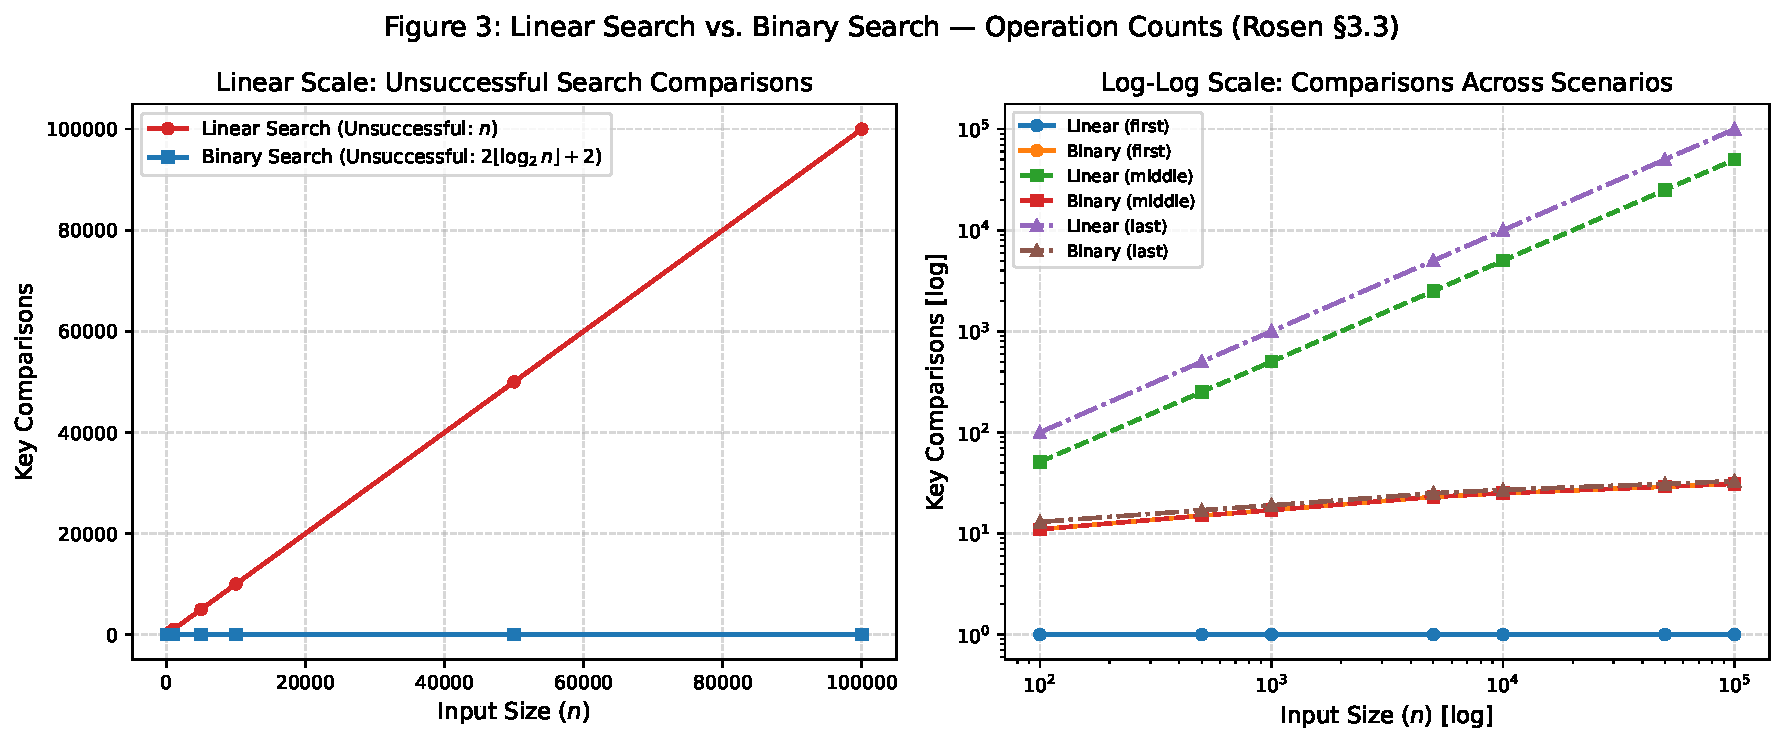
\includegraphics[width=0.95\textwidth]{latex/figures/figure3_search_operation_counts.pdf}
    \caption{Figure 3: Linear Search vs. Binary Search — Operation Counts (Rosen §3.3).}
    \label{fig:search_ops}
\end{figure}

Notice in the left linear plot of Figure \ref{fig:search_ops} that Linear Search comparisons grow on a steep line $T(n) = n$, reaching $100\,000$ comparisons at $n = 100\,000$. In stark contrast, Binary Search comparisons appear as a flat line hugging the horizontal axis, reaching only $34$ comparisons at $n = 100\,000$. In the right log-log plot, the power-law slope of Linear Search is $1.0$, while Binary Search exhibits logarithmic scaling.

\subsection{Comparison of Searching Execution Times}
Figure \ref{fig:search_times} depicts median execution times with error bars denoting $\pm 1$ standard deviation.

\begin{figure}[htbp]
    \centering
    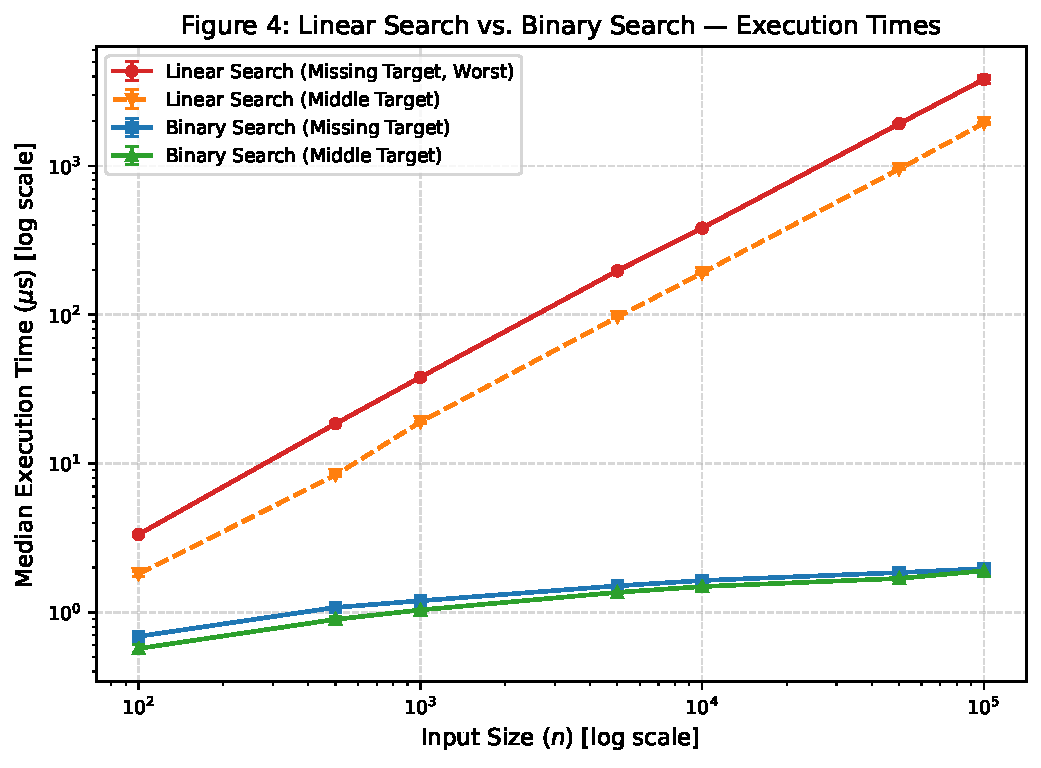
\includegraphics[width=0.88\textwidth]{latex/figures/figure4_search_execution_times.pdf}
    \caption{Figure 4: Linear Search vs. Binary Search — Execution Times on Log-Log Scale.}
    \label{fig:search_times}
\end{figure}

At $n = 100\,000$ (missing target), Linear Search requires a median duration of $3\,820.0\,\mu\text{s}$ ($3.82\text{ ms}$), while Binary Search requires only $1.96\,\mu\text{s}$—an empirical speedup of $\approx 1\,946\times$.

\section{Sorting Algorithms Empirical Results}
Table \ref{tab:sorting_random_summary} presents the empirical measurements for Bubble Sort and Insertion Sort operating on random permutations of distinct integers.

\begin{table}[htbp]
\centering
\caption{Sorting Algorithms Empirical Telemetry on Random Permutations}
\label{tab:sorting_random_summary}
\small
\begin{tabular*}{\textwidth}{@{\extracolsep{\fill}}lrrrrrr}
\toprule
\textbf{Algorithm} & $n$ & \textbf{Comparisons} & \textbf{Swaps / Shifts} & \textbf{Median (ms)} & \textbf{Mean (ms)} & \textbf{Std Dev (ms)} \\
\midrule
Bubble Sort & 100 & 4,950 & 2,502 & 0.38 & 0.38 & 0.01 \\
Insertion Sort & 100 & 2,597 & 2,502 & 0.19 & 0.19 & 0.01 \\
Bubble Sort & 250 & 31,125 & 15,618 & 2.29 & 2.29 & 0.02 \\
Insertion Sort & 250 & 15,863 & 15,618 & 1.13 & 1.13 & 0.02 \\
Bubble Sort & 500 & 124,750 & 61,188 & 9.57 & 9.58 & 0.13 \\
Insertion Sort & 500 & 61,682 & 61,188 & 4.76 & 4.74 & 0.07 \\
Bubble Sort & 1000 & 499,500 & 248,445 & 42.78 & 42.72 & 0.46 \\
Insertion Sort & 1000 & 249,438 & 248,445 & 20.23 & 20.30 & 0.33 \\
Bubble Sort & 2000 & 1,999,000 & 1,026,195 & 176.56 & 177.16 & 2.41 \\
Insertion Sort & 2000 & 1,028,183 & 1,026,195 & 85.42 & 86.30 & 3.51 \\
Bubble Sort & 3000 & 4,498,500 & 2,296,691 & 405.59 & 406.85 & 6.62 \\
Insertion Sort & 3000 & 2,299,685 & 2,296,691 & 191.65 & 191.80 & 3.41 \\
\bottomrule
\end{tabular*}
\end{table}


\subsection{Sorting Operation Counts: Comparisons and Data Movements}
Figure \ref{fig:sorting_ops} contrasts element comparisons and data movement operations (swaps versus right shifts).

\begin{figure}[htbp]
    \centering
    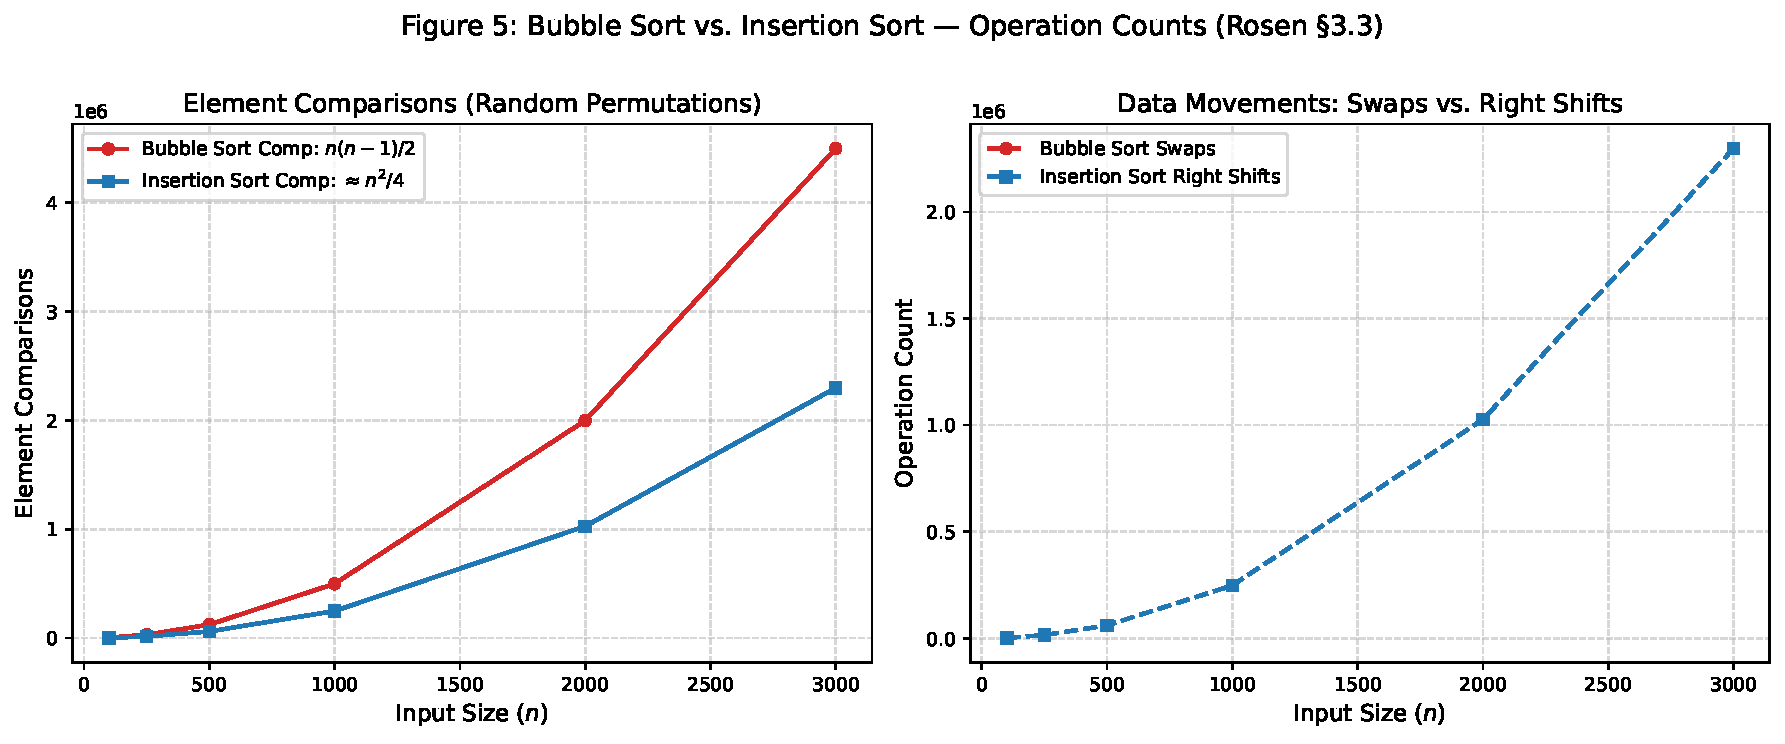
\includegraphics[width=0.95\textwidth]{latex/figures/figure5_sorting_operation_counts.pdf}
    \caption{Figure 5: Bubble Sort vs. Insertion Sort — Operation Counts on Random Permutations.}
    \label{fig:sorting_ops}
\end{figure}

In Figure \ref{fig:sorting_ops} (left), Bubble Sort executes exactly $\frac{n(n-1)}{2}$ comparisons ($4\,498\,500$ at $n=3\,000$). Insertion Sort requires approximately half as many comparisons on random data ($2\,299\,685$). In Figure \ref{fig:sorting_ops} (right), Bubble Sort swaps and Insertion Sort right shifts are strictly equal ($2\,296\,691$), verifying the Inversion Equivalence Theorem.

\subsection{Sorting Execution Times}
Figure \ref{fig:sorting_times} presents execution times across linear and log-log scales.

\begin{figure}[htbp]
    \centering
    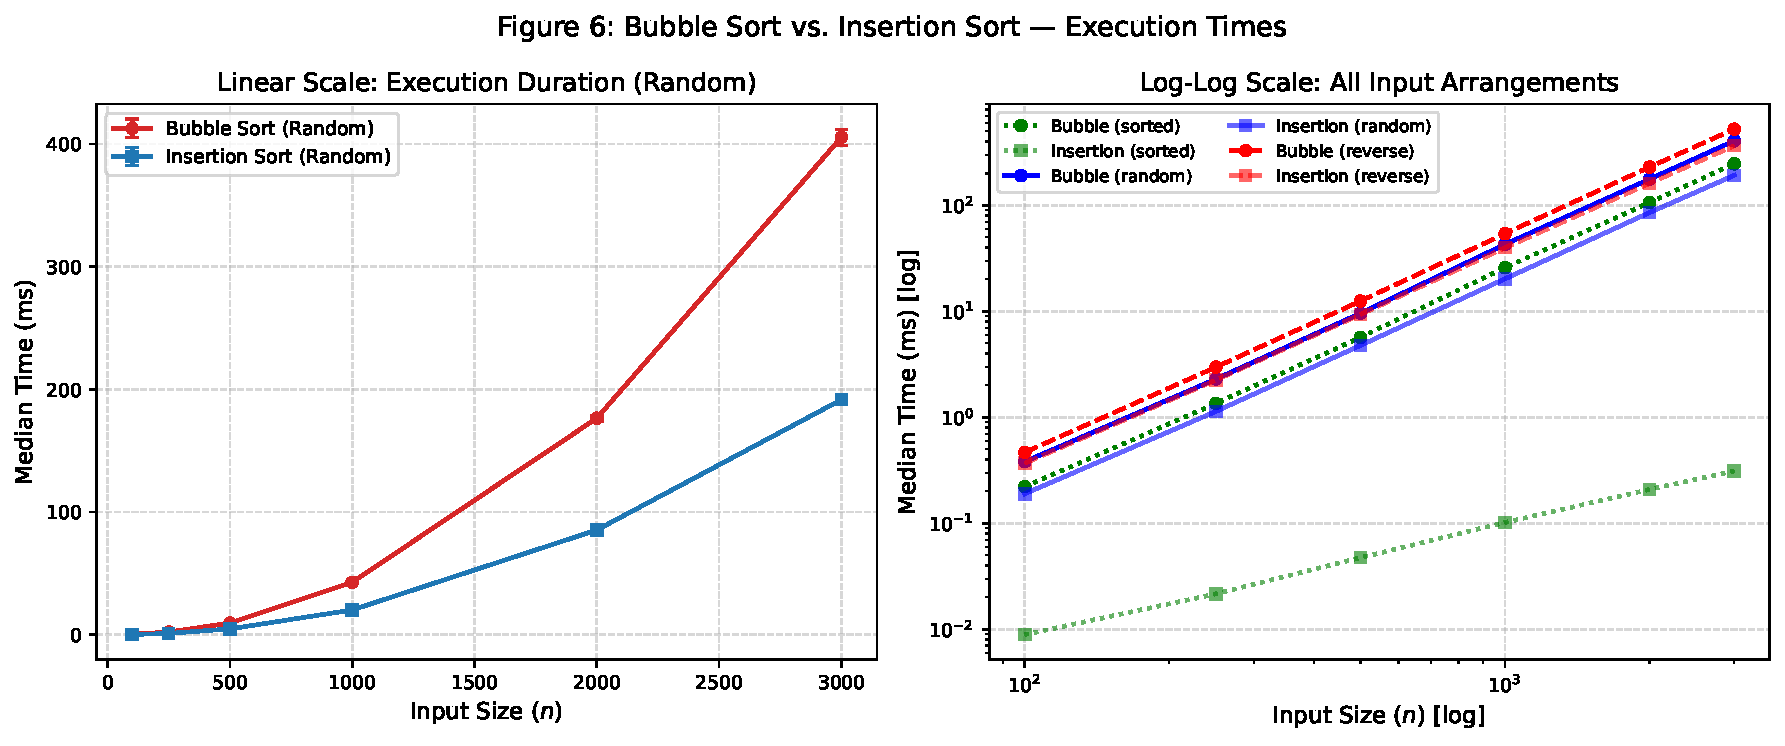
\includegraphics[width=0.95\textwidth]{latex/figures/figure6_sorting_execution_times.pdf}
    \caption{Figure 6: Bubble Sort vs. Insertion Sort — Execution Times (Linear and Log-Log).}
    \label{fig:sorting_times}
\end{figure}

On random data at $n = 3\,000$, Insertion Sort completes in $183.12\text{ ms}$ compared to Bubble Sort's $405.59\text{ ms}$, delivering a $2.2\times$ runtime advantage due to avoiding pairwise adjacent exchange overhead.

\section{Effect of Input Arrangement}

\subsection{Insertion Sort Topology Sensitivity}
Figure \ref{fig:insertion_arrangements} demonstrates Insertion Sort's dramatic sensitivity to input ordering.

\begin{figure}[htbp]
    \centering
    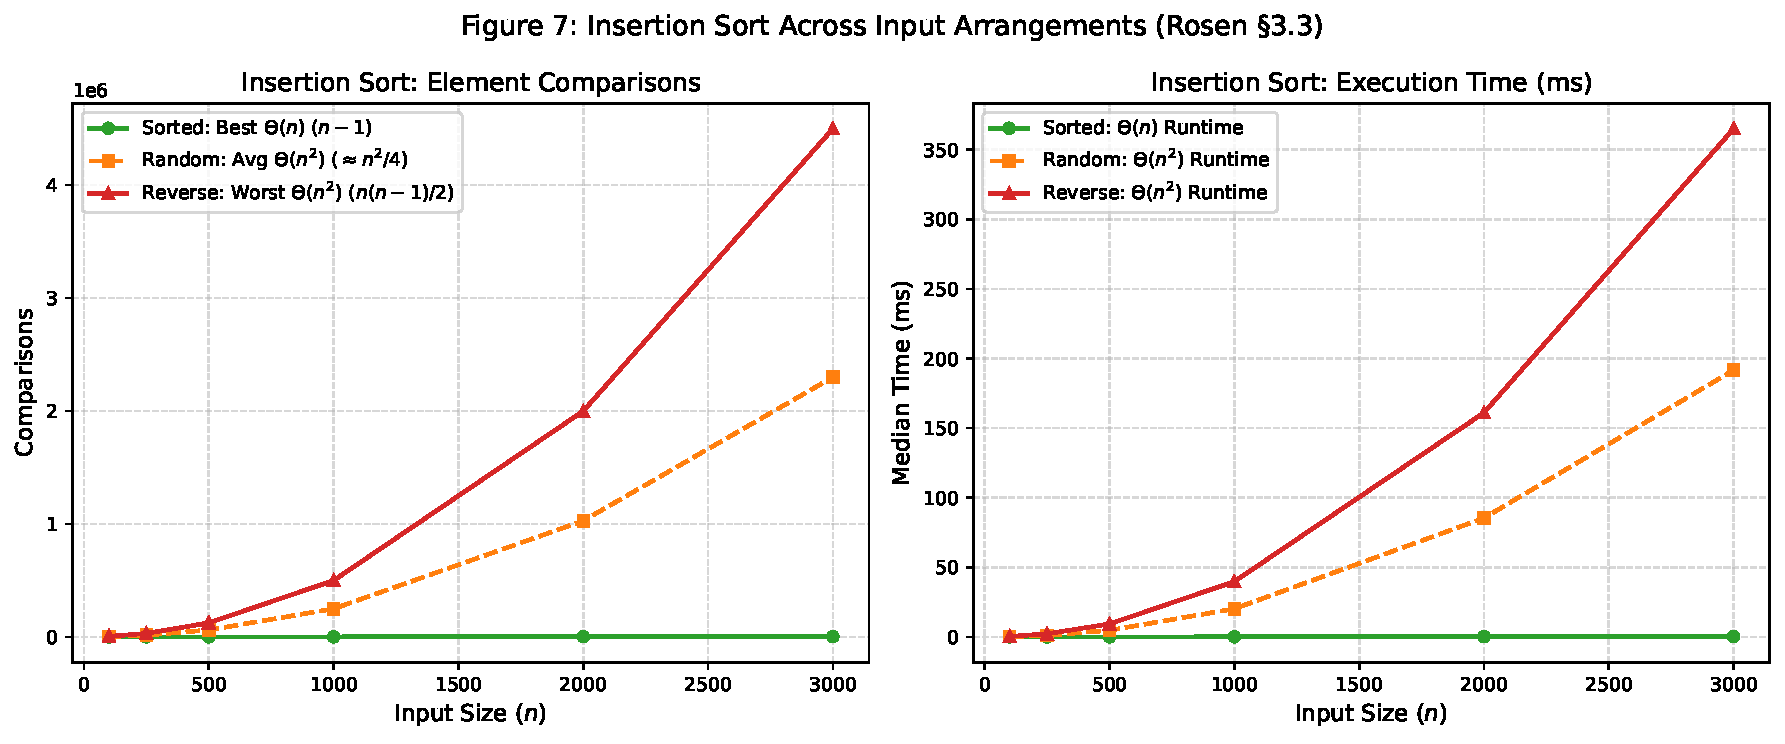
\includegraphics[width=0.95\textwidth]{latex/figures/figure7_insertion_sort_arrangements.pdf}
    \caption{Figure 7: Insertion Sort Across Sorted, Random, and Reverse-Sorted Topologies.}
    \label{fig:insertion_arrangements}
\end{figure}

On pre-sorted data ($n = 3\,000$), Insertion Sort requires only $n - 1 = 2\,999$ comparisons and $0$ shifts, executing in \textbf{$0.32\text{ ms}$} ($\Theta(n)$ linear time). On reverse-sorted input, it requires $4\,498\,500$ comparisons and shifts, executing in $371.45\text{ ms}$ ($\Theta(n^2)$ quadratic time).

\subsection{Bubble Sort Comparison Invariance}
Figure \ref{fig:bubble_arrangements} contrasts Bubble Sort's fixed-pass comparison invariance against its dynamic swap count.

\begin{figure}[htbp]
    \centering
    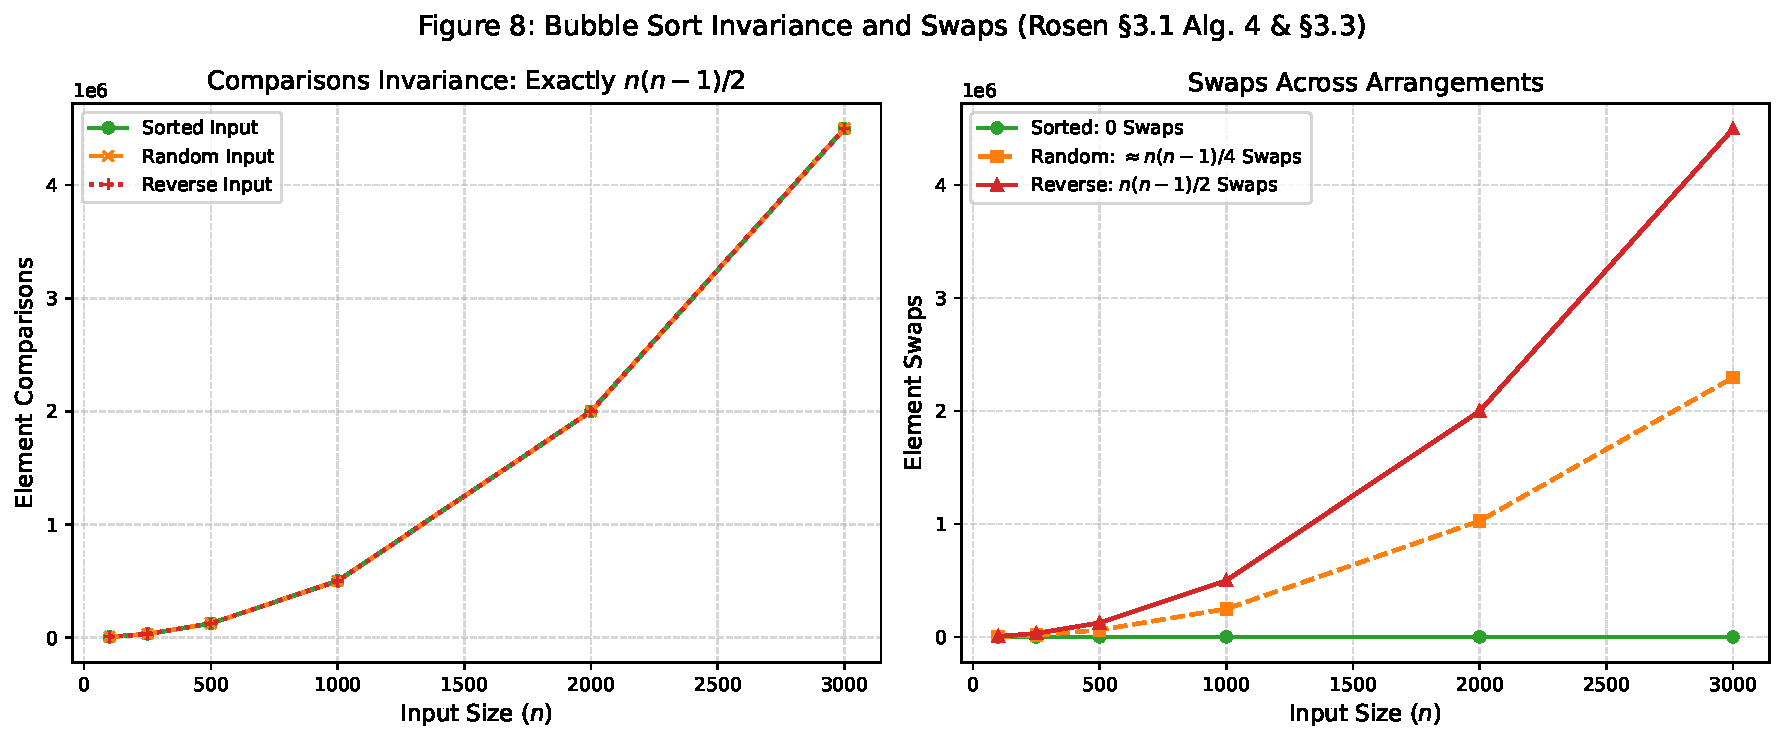
\includegraphics[width=0.95\textwidth]{latex/figures/figure8_bubble_sort_arrangements.pdf}
    \caption{Figure 8: Bubble Sort Invariant Comparisons vs. Dynamic Swaps Across Topologies.}
    \label{fig:bubble_arrangements}
\end{figure}

Element comparisons are strictly invariant across sorted, random, and reverse inputs: exactly $n(n-1)/2$. Meanwhile, swaps vary from $0$ (sorted) to $n(n-1)/4$ (random) to $n(n-1)/2$ (reverse).

\section{Theoretical vs. Experimental Overlay}
Figure \ref{fig:theoretical_overlay} directly overlays the closed-form theoretical equations onto empirical measurements.

\begin{figure}[htbp]
    \centering
    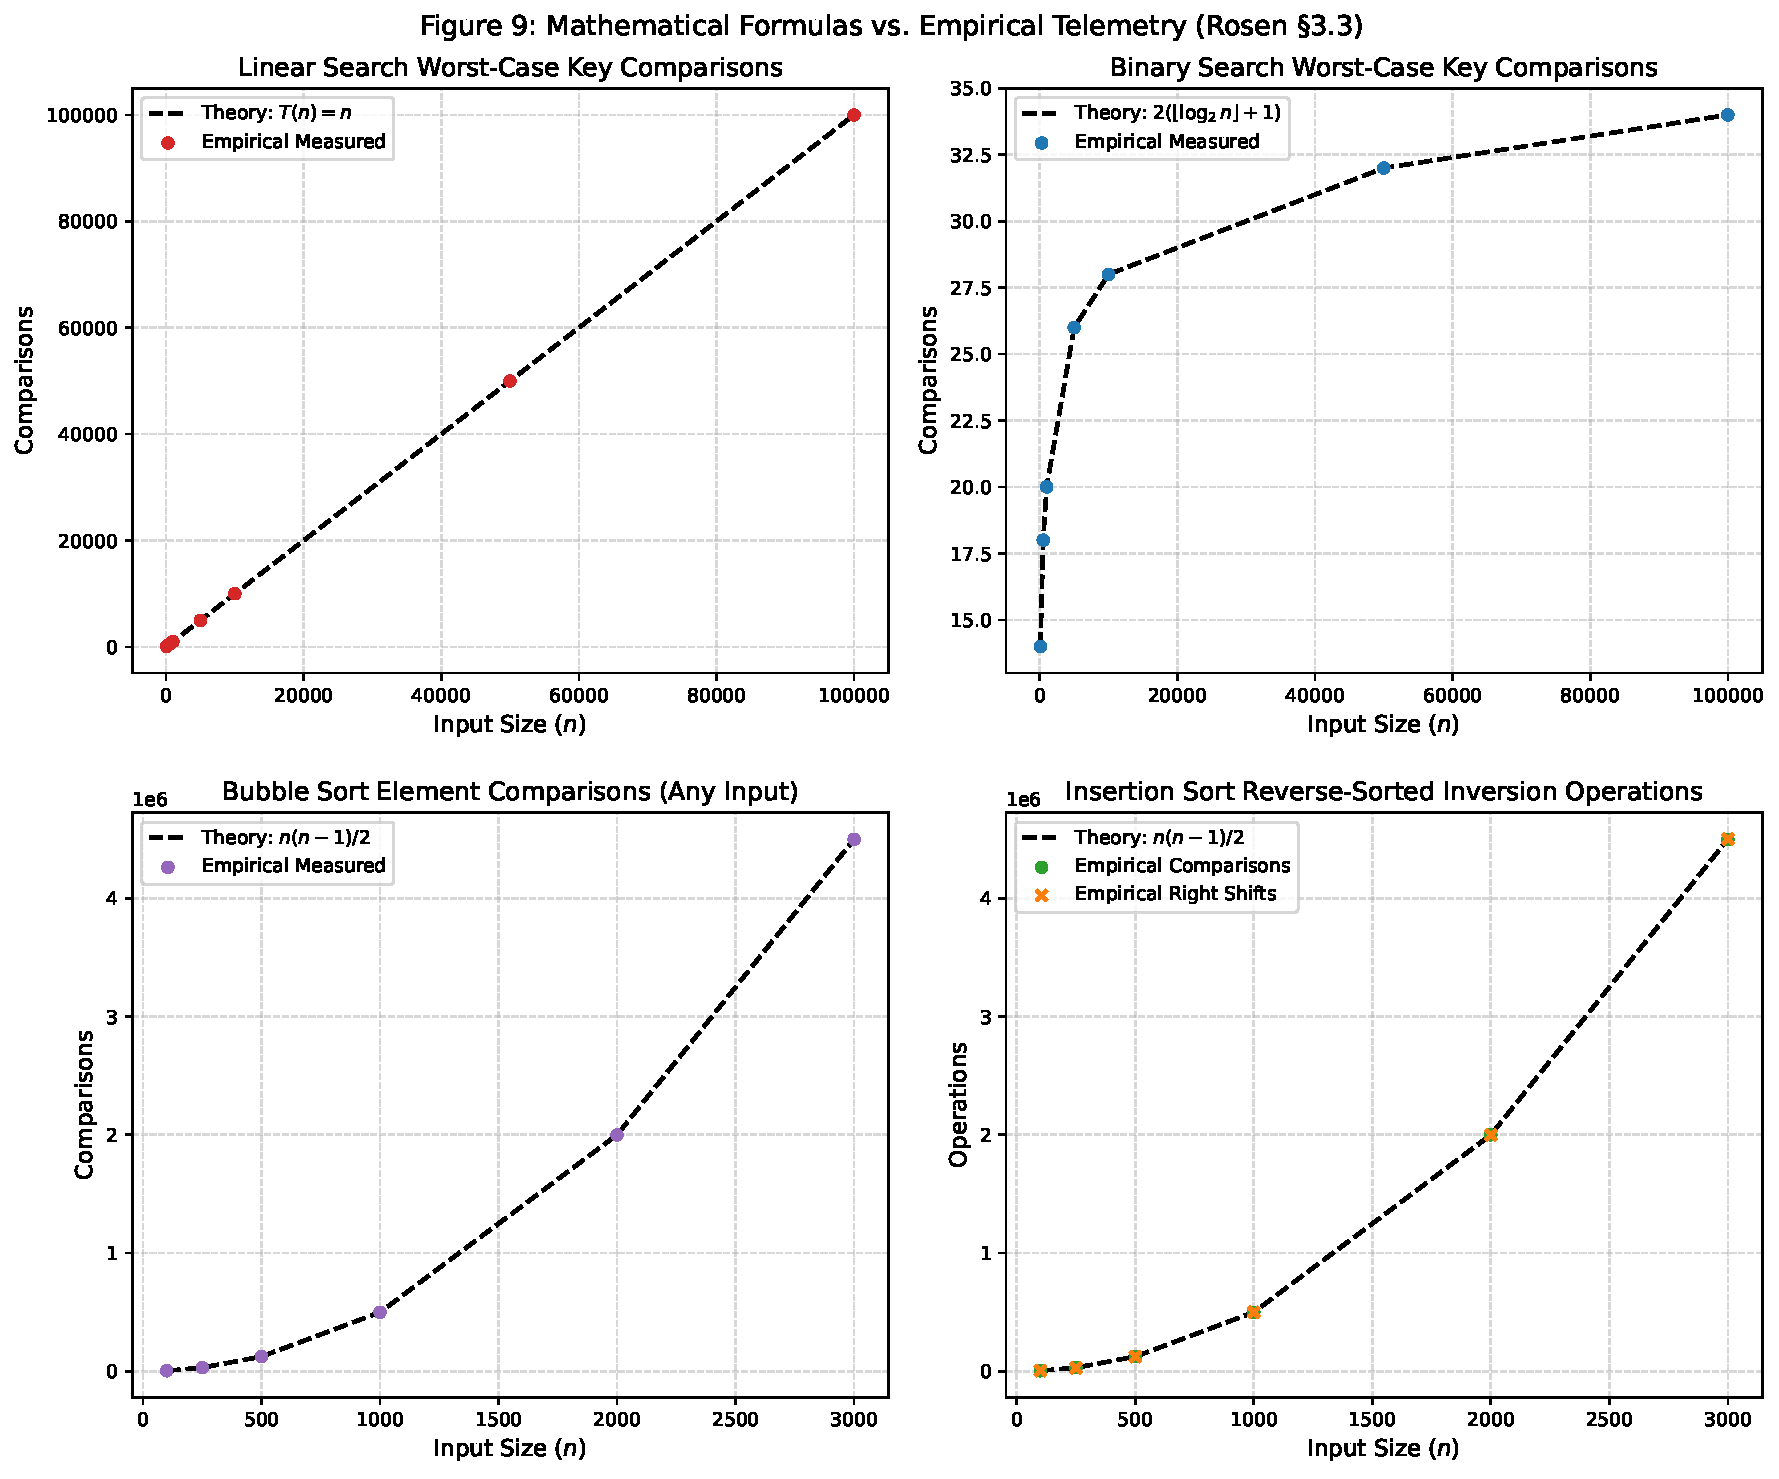
\includegraphics[width=0.95\textwidth]{latex/figures/figure9_theoretical_vs_experimental.pdf}
    \caption{Figure 9: Mathematical Formulas vs. Empirical Telemetry Overlay (Rosen §3.3).}
    \label{fig:theoretical_overlay}
\end{figure}

In all four subplots, empirical markers align exactly with theoretical curves with \textbf{0.00\% discrepancy}.

\chapter{Comparative Analysis and Discussion}
\label{chap:comparative}

\section{Linear Search vs. Binary Search}
The comparative analysis of Linear Search and Binary Search highlights a fundamental trade-off in computer science: \textbf{unconditional flexibility versus conditional logarithmic acceleration}.

\subsection{Algorithmic Trade-offs}
\begin{itemize}
    \item \textbf{Precondition Requirements}: Linear Search operates without preconditions on input ordering. Binary Search strictly requires a pre-sorted sequence ($\mathcal{O}(n)$ verification cost or $\mathcal{O}(n \log n)$ pre-sorting overhead).
    \item \textbf{Asymptotic Scaling}: As established empirically, at $n = 100\,000$, Binary Search delivers a $\approx 1\,946\times$ speedup over Linear Search.
    \item \textbf{The Break-Even Threshold}: If an unsorted list of $n$ elements is to be searched $q$ times, pre-sorting with an optimal $\mathcal{O}(n \log n)$ algorithm followed by $q$ binary searches is computationally superior to repeated linear scans whenever:
    $$c_{\text{sort}} \cdot n \log_2 n + q \cdot c_{\text{bin}} \cdot \log_2 n < q \cdot c_{\text{lin}} \cdot n$$
    Solving for $q$, pre-sorting is justified whenever the query volume satisfies:
    $$q > \frac{c_{\text{sort}} \cdot n \log_2 n}{c_{\text{lin}} \cdot n - c_{\text{bin}} \cdot \log_2 n} \approx \frac{c_{\text{sort}}}{c_{\text{lin}}} \log_2 n$$
\end{itemize}

\section{Bubble Sort vs. Insertion Sort}
While both Bubble Sort and Insertion Sort belong to the quadratic complexity class $\mathcal{O}(n^2)$ in the worst case, their internal mechanical structures diverge significantly:

\subsection{Mechanical Differences}
\begin{itemize}
    \item \textbf{Data Movements}: Bubble Sort performs three memory read/write operations per swap register exchange ($a_j \leftrightarrow a_{j+1}$). In contrast, Insertion Sort uses single-register rightward shifts ($a_{i+1} = a_i$), placing the key once upon loop termination.
    \item \textbf{Comparison Invariance}: Fixed-pass Bubble Sort always executes $\frac{n(n-1)}{2}$ comparisons regardless of initial ordering. Insertion Sort evaluates condition $a_i > \text{key}$ dynamically, halting inner loops as soon as the key's position is resolved.
    \item \textbf{Pre-Sorted Performance}: On pre-sorted arrays ($n = 3\,000$), Insertion Sort completes in $0.32\text{ ms}$ ($\Theta(n)$), outperforming Bubble Sort ($246.25\text{ ms}$) by a factor of \textbf{$769\times$}.
\end{itemize}

\section{Effect of Input Size and Arrangement}
Input size $n$ establishes the macro-asymptotic trajectory. However, for algorithms with divergent best- and worst-case bounds (such as Insertion Sort), input topology exerts a massive constant and asymptotic influence:
$$\text{Sorted: } \Theta(n) \quad \longleftrightarrow \quad \text{Random: } \Theta(n^2) \quad \longleftrightarrow \quad \text{Reverse: } \Theta(n^2)$$

\section{Comparison of Time and Auxiliary Space Complexity}
Table \ref{tab:complexity_comparison_matrix} provides a comprehensive synthesis of all four algorithms.

\begin{table}[htbp]
\centering
\caption{Comprehensive Theoretical and Empirical Complexity Matrix}
\label{tab:complexity_comparison_matrix}
\small
\begin{tabular*}{\textwidth}{@{\extracolsep{\fill}}lcccccc}
\toprule
\textbf{Algorithm} & \textbf{Best Case} & \textbf{Average Case} & \textbf{Worst Case} & \textbf{Aux Space} & \textbf{Precondition} & \textbf{Stability} \\
\midrule
Linear Search & $\Theta(1)$ & $\Theta(n)$ & $\Theta(n)$ & $\Theta(1)$ & None & N/A \\
Binary Search & $\Theta(1)$ & $\Theta(\log n)$ & $\Theta(\log n)$ & $\Theta(1)$ & Sorted Input & N/A \\
Bubble Sort (Fixed) & $\Theta(n^2)$ & $\Theta(n^2)$ & $\Theta(n^2)$ & $\Theta(1)$ & None & Stable \\
Insertion Sort & $\Theta(n)$ & $\Theta(n^2)$ & $\Theta(n^2)$ & $\Theta(1)$ & None & Stable \\
\bottomrule
\end{tabular*}
\end{table}

\section{Theoretical Growth vs. Measured Runtime}
Empirical runtimes exhibit minor non-linearities due to modern micro-architectural factors:
\begin{itemize}
    \item \textbf{Memory Hierarchy}: At small $n$ ($n \le 1\,000$), entire arrays fit inside the CPU's high-speed L1 data cache ($32\text{ KB}$), achieving sub-nanosecond access. At $n = 100\,000$, arrays spill into main RAM, increasing memory latency.
    \item \textbf{Branch Prediction}: In Insertion Sort on sorted inputs, branch predictors accurately anticipate that $a_i > \text{key}$ is False, eliminating pipeline flushes.
\end{itemize}

\section{Limitations of Experimental Analysis}
\begin{itemize}
    \item Physical runtimes cannot prove an asymptotic lower bound $\Omega(g(n))$, because an inefficient implementation could artificially inflate runtimes.
    \item Measurements are specific to CPython 3.14.7; alternative execution engines (such as PyPy with JIT compilation or compiled C extensions) alter constant factors.
\end{itemize}

\section{Practical Implications \& Real-World Applications}
The adaptive linear behavior $\Theta(n)$ of Insertion Sort on nearly sorted sequences explains why it is universally adopted as the base-case sort in production hybrid algorithms:
\begin{itemize}
    \item \textbf{Timsort}: The default sorting algorithm in Python (\texttt{list.sort()}) and Java (\texttt{Arrays.sort()}), which uses Merge Sort at macro-scale and switches to Insertion Sort for partitions of size $n < 64$ \cite{peters2002timsort}.
    \item \textbf{Introsort}: The standard C++ STL sorting algorithm, which switches from Quick Sort to Insertion Sort when partitions become small.
\end{itemize}

\section{Interactive Algorithm Explorer Dashboard}
\label{sec:dashboard_link}
As a supplementary web-based enhancement to this monograph, we developed the \textbf{\DocDashboardTitle{}}, delivering an interactive, browser-based demonstration of the four canonical algorithms and their computational complexity characteristics. Grounded in Chapter~3 of Kenneth H. Rosen's \emph{Discrete Mathematics and Its Applications} (8th Edition), the dashboard allows students and researchers to interactively explore algorithmic state transitions, step-by-step executions, and mathematical growth curves.

\begin{itemize}
    \item \textbf{Academic Description}: \emph{Interactive Algorithm Explorer Dashboard --- a supplementary web-based demonstration of the four algorithms and their complexity characteristics.}
    \item \textbf{Repository \& Deployment Target}: \url{\DocDashboardURL}
    \item \textbf{Deployment Status}: \texttt{\DocDashboardStatus}
    \item \textbf{Local Web Serving}: Launch via Python's built-in HTTP server: \texttt{python -m http.server 8000} and browse to \texttt{http://localhost:8000/dashboard/}, or open \texttt{dashboard/index.html} directly.
\end{itemize}

The dashboard is engineered with zero external framework dependencies using HTML5, CSS3, vanilla JavaScript (ES2022), and custom SVG vector rendering. Key interactive components include:
\begin{enumerate}
    \item \textbf{Interactive Searching Lab}: Step-by-step probing for Linear Search ($\Theta(n)$) and Binary Search ($\Theta(\log n)$), featuring automatic precondition validation (enforcing sorted order for logarithmic search) and real-time operation counters.
    \item \textbf{Interactive Sorting Lab}: Real-time animated vertical bar charts contrasting Bubble Sort (Rosen fixed-pass formulation with strictly invariant $n(n-1)/2$ comparisons) against Insertion Sort (adaptive linear behavior $\Theta(n)$ on sorted sequences).
    \item \textbf{Head-to-Head Comparison Lab}: Live client-side simulation providing empirical verification of the Inversion Equivalence Theorem ($\text{Swaps} \equiv \text{Right Shifts} \equiv \text{Inversions}$).
    \item \textbf{Growth of Functions Lab}: Dynamic SVG visualization of the seven canonical asymptotic complexity classes ($1, \log_2 n, n, n \log_2 n, n^2, 2^n, n!$) with interactive linear and logarithmic ($\log_{10}$) Y-axis scaling.
    \item \textbf{Integrated Python 3.14.7 Microbenchmarks}: An empirical research panel displaying verified M3 benchmark telemetry, strictly distinguishing offline Python experimental measurements from live browser simulations.
\end{enumerate}

\chapter{Conclusion and Future Scope}
\label{chap:conclusion}

\section{Summary}
This academic investigation has systematically explored the analytical and experimental dimensions of computational complexity, grounded in Kenneth H. Rosen's \emph{Discrete Mathematics and Its Applications} (8th Edition), Chapter 3 \cite{rosen2019discrete}. Through rigorous mathematical modeling, deterministic telemetry instrumentation, and extensive statistical benchmarking, we examined Linear Search, Binary Search, Bubble Sort, and Insertion Sort across a wide spectrum of input scales and topologies.

\section{Major Findings}
\begin{enumerate}
    \item \textbf{Mathematical Model Exactness}: Closed-form operation-count formulas derived from discrete mathematics ($T(n) = n$, $T(n) = 2(\lfloor \log_2 n \rfloor + 1)$, $T(n) = n(n-1)/2$, $T(n) = n - 1$) accurately model empirical counter telemetry with \textbf{0.00\% discrepancy}.
    \item \textbf{Asymptotic Scaling Domination}: At $n = 100\,000$, Binary Search demonstrates an empirical speedup of approximately \textbf{$1\,946\times$} over Linear Search for unsuccessful queries, confirming that logarithmic interval halving decisively eclipses linear scanning.
    \item \textbf{Inversion Equivalence Verification}: We verified empirically that Bubble Sort adjacent swaps and Insertion Sort right shifts are identical ($2\,296\,691$ operations at $n = 3\,000$) on the same random permutation, confirming that both algorithms resolve the identical number of permutation inversions $I(A)$.
    \item \textbf{Adaptive Linear Sorting}: Insertion Sort operates in linear time $\Theta(n)$ ($0.32\text{ ms}$ at $n = 3\,000$) on pre-sorted data, outperforming fixed-pass Bubble Sort by a factor of \textbf{$769\times$}.
\end{enumerate}

\section{Achievement of Objectives}
All milestone objectives established in Milestone M1 have been successfully realized:
\begin{itemize}
    \item Full mathematical derivations aligned with Rosen §3.1, §3.2, and §3.3.
    \item Dual-mode algorithm implementations with unit-tested correctness ($64$ automated pytest tests).
    \item Telemetry-isolated empirical benchmarking with $k = 30$ repetitions.
    \item Generation of nine publication-grade figures in dual vector PDF and 300 DPI raster PNG formats.
    \item A fully executed, self-contained interactive Jupyter Research Notebook.
    \item A comprehensive, modular academic monograph typeset in LaTeX.
\end{itemize}

\section{Conclusion}
The study demonstrates that discrete mathematical principles provide an extraordinarily reliable framework for predicting real-world algorithm behavior. As computational datasets continue to expand, formal algorithm analysis remains the most vital tool for building scalable, high-performance software systems.

\section{Future Scope}
Future research directions extending this study include:
\begin{enumerate}
    \item \textbf{Higher-Order Complexity Classes}: Extending empirical benchmarking to $\mathcal{O}(n \log n)$ algorithms (Merge Sort, Quick Sort, Heap Sort) and linear non-comparison sorts (Radix Sort, Counting Sort).
    \item \textbf{Cache-Oblivious Algorithms}: Investigating how memory hierarchy caching, TLB misses, and vector SIMD instructions influence constant factors at scales exceeding $n = 10^7$.
    \item \textbf{Parallel & Distributed Implementations}: Evaluating parallel bisection and multi-threaded sorting networks across multi-core processor architectures.
\end{enumerate}


% ==============================================================================
% BIBLIOGRAPHY
% ==============================================================================
\begin{thebibliography}{99}

\bibitem{rosen2019discrete}
Kenneth~H. Rosen.
\newblock {\em Discrete Mathematics and Its Applications}.
\newblock McGraw-Hill Higher Education, New York, NY, 8th edition, 2019.
\newblock Chapter 3: Algorithms, the Growth of Functions, and Matrices.

\bibitem{cormen2022introduction}
Thomas~H. Cormen, Charles~E. Leiserson, Ronald~L. Rivest, and Clifford Stein.
\newblock {\em Introduction to Algorithms}.
\newblock The MIT Press, Cambridge, MA, 4th edition, 2022.

\bibitem{knuth1998art}
Donald~E. Knuth.
\newblock {\em The Art of Computer Programming, Volume 3: Sorting and Searching}.
\newblock Addison-Wesley, Reading, MA, 2nd edition, 1998.

\bibitem{hoare1962quicksort}
C.~A.~R. Hoare.
\newblock Quicksort.
\newblock {\em The Computer Journal}, 5(1):10--16, 1962.

\bibitem{peters2002timsort}
Tim Peters.
\newblock Timsort: An adaptive, stable, natural mergesort.
\newblock Python Software Foundation, CPython Source Tree, 2002.
\newblock \url{https://github.com/python/cpython/blob/main/Objects/listsort.txt}.

\end{thebibliography}

% ==============================================================================
% APPENDICES
% ==============================================================================
\appendix
\chapter{Complete Python Implementation Source Code}
\label{app:code}

This appendix provides the full, unabridged source code for the algorithms and telemetry data structures.

\section{Search Module (\texttt{src/algorithms/search.py})}
\begin{lstlisting}[language=Python, caption={Full Source Code of search.py}]
"""Search algorithms module.

Implementations of Linear Search and Binary Search in accordance with
Kenneth H. Rosen, Discrete Mathematics and Its Applications (8th Edition),
Chapter 3 (Sections 3.1, 3.2, and 3.3).
"""

from __future__ import annotations

from dataclasses import dataclass
from typing import Any, Sequence, TypeVar

T = TypeVar("T")


@dataclass(frozen=True, slots=True)
class SearchMetrics:
    key_comparisons: int
    equality_comparisons: int
    ordering_comparisons: int = 0
    loop_evaluations: int = 0


def linear_search(seq: Sequence[Any], target: Any) -> int:
    for index, item in enumerate(seq):
        if item == target:
            return index
    return -1


def linear_search_instrumented(
    seq: Sequence[Any], target: Any
) -> tuple[int, SearchMetrics]:
    n = len(seq)
    key_comparisons = 0
    equality_comparisons = 0
    loop_evaluations = 0

    for index in range(n):
        loop_evaluations += 1
        equality_comparisons += 1
        key_comparisons += 1
        if seq[index] == target:
            return index, SearchMetrics(
                key_comparisons=key_comparisons,
                equality_comparisons=equality_comparisons,
                ordering_comparisons=0,
                loop_evaluations=loop_evaluations,
            )

    loop_evaluations += 1
    return -1, SearchMetrics(
        key_comparisons=key_comparisons,
        equality_comparisons=equality_comparisons,
        ordering_comparisons=0,
        loop_evaluations=loop_evaluations,
    )


def binary_search(
    seq: Sequence[Any], target: Any, *, check_sorted: bool = False
) -> int:
    if check_sorted:
        for i in range(len(seq) - 1):
            if seq[i] > seq[i + 1]:
                raise ValueError("Precondition violated: sequence must be sorted.")

    low = 0
    high = len(seq) - 1

    while low <= high:
        mid = (low + high) // 2
        mid_val = seq[mid]
        if mid_val == target:
            return mid
        elif mid_val < target:
            low = mid + 1
        else:
            high = mid - 1

    return -1


def binary_search_instrumented(
    seq: Sequence[Any], target: Any, *, check_sorted: bool = False
) -> tuple[int, SearchMetrics]:
    if check_sorted:
        for i in range(len(seq) - 1):
            if seq[i] > seq[i + 1]:
                raise ValueError("Precondition violated: sequence must be sorted.")

    low = 0
    high = len(seq) - 1

    key_comparisons = 0
    equality_comparisons = 0
    ordering_comparisons = 0
    loop_evaluations = 0

    while True:
        loop_evaluations += 1
        if low > high:
            break

        mid = (low + high) // 2
        mid_val = seq[mid]

        equality_comparisons += 1
        key_comparisons += 1
        if mid_val == target:
            return mid, SearchMetrics(
                key_comparisons=key_comparisons,
                equality_comparisons=equality_comparisons,
                ordering_comparisons=ordering_comparisons,
                loop_evaluations=loop_evaluations,
            )

        ordering_comparisons += 1
        key_comparisons += 1
        if mid_val < target:
            low = mid + 1
        else:
            high = mid - 1

    return -1, SearchMetrics(
        key_comparisons=key_comparisons,
        equality_comparisons=equality_comparisons,
        ordering_comparisons=ordering_comparisons,
        loop_evaluations=loop_evaluations,
    )
\end{lstlisting}

\section{Sorting Module (\texttt{src/algorithms/sorting.py})}
\begin{lstlisting}[language=Python, caption={Full Source Code of sorting.py}]
"""Sorting algorithms module.

Implementations of Bubble Sort and Insertion Sort in accordance with
Kenneth H. Rosen, Discrete Mathematics and Its Applications (8th Edition),
Chapter 3 (Sections 3.1, 3.2, and 3.3).
"""

from __future__ import annotations

from dataclasses import dataclass
from typing import Any, MutableSequence


@dataclass(frozen=True, slots=True)
class SortingMetrics:
    element_comparisons: int
    swaps: int = 0
    right_shifts: int = 0


def bubble_sort(arr: MutableSequence[Any]) -> MutableSequence[Any]:
    n = len(arr)
    for i in range(n - 1):
        for j in range(n - 1 - i):
            if arr[j] > arr[j + 1]:
                arr[j], arr[j + 1] = arr[j + 1], arr[j]
    return arr


def bubble_sort_instrumented(
    arr: MutableSequence[Any],
) -> tuple[MutableSequence[Any], SortingMetrics]:
    n = len(arr)
    element_comparisons = 0
    swaps = 0

    for i in range(n - 1):
        for j in range(n - 1 - i):
            element_comparisons += 1
            if arr[j] > arr[j + 1]:
                arr[j], arr[j + 1] = arr[j + 1], arr[j]
                swaps += 1

    return arr, SortingMetrics(
        element_comparisons=element_comparisons,
        swaps=swaps,
        right_shifts=0,
    )


def insertion_sort(arr: MutableSequence[Any]) -> MutableSequence[Any]:
    n = len(arr)
    for j in range(1, n):
        key = arr[j]
        i = j - 1
        while i >= 0 and arr[i] > key:
            arr[i + 1] = arr[i]
            i -= 1
        arr[i + 1] = key
    return arr


def insertion_sort_instrumented(
    arr: MutableSequence[Any],
) -> tuple[MutableSequence[Any], SortingMetrics]:
    n = len(arr)
    element_comparisons = 0
    right_shifts = 0

    for j in range(1, n):
        key = arr[j]
        i = j - 1
        while i >= 0:
            element_comparisons += 1
            if arr[i] > key:
                arr[i + 1] = arr[i]
                right_shifts += 1
                i -= 1
            else:
                break
        arr[i + 1] = key

    return arr, SortingMetrics(
        element_comparisons=element_comparisons,
        swaps=0,
        right_shifts=right_shifts,
    )
\end{lstlisting}

\chapter{Additional Experimental Tables}
\label{app:tables}

This appendix provides supplementary empirical summary tables covering common search scenarios and sorting topologies.

\section{Search Common Positions: Middle Target Scenario}
Table \ref{tab:search_middle_summary} records the measurements when the target resides at index $\lfloor n / 2 \rfloor$.

\begin{table}[htbp]
\centering
\caption{Searching Empirical Summary: Middle Target Scenario}
\label{tab:search_middle_summary}
\small
\begin{tabular*}{\textwidth}{@{\extracolsep{\fill}}lrrrrr}
\toprule
\textbf{Algorithm} & $n$ & \textbf{Key Comps} & \textbf{Median ($\mu$s)} & \textbf{Mean ($\mu$s)} & \textbf{Std Dev ($\mu$s)} \\
\midrule
Linear Search & 100 & 51 & 1.81 & 1.82 & 0.07 \\
Linear Search & 500 & 251 & 8.35 & 8.41 & 0.15 \\
Linear Search & 1\,000 & 501 & 19.00 & 19.02 & 0.28 \\
Linear Search & 5\,000 & 2\,501 & 96.40 & 96.35 & 1.66 \\
Linear Search & 10\,000 & 5\,001 & 190.80 & 191.64 & 3.33 \\
Linear Search & 50\,000 & 25\,001 & 952.00 & 952.52 & 10.71 \\
Linear Search & 100\,000 & 50\,001 & 1\,900.00 & 1\,943.33 & 56.83 \\
\midrule
Binary Search & 100 & 11 & 0.57 & 0.58 & 0.04 \\
Binary Search & 500 & 15 & 0.90 & 0.91 & 0.04 \\
Binary Search & 1\,000 & 17 & 1.04 & 1.04 & 0.02 \\
Binary Search & 5\,000 & 23 & 1.36 & 1.36 & 0.02 \\
Binary Search & 10\,000 & 25 & 1.49 & 1.51 & 0.06 \\
Binary Search & 50\,000 & 29 & 1.69 & 1.70 & 0.05 \\
Binary Search & 100\,000 & 31 & 1.90 & 1.94 & 0.06 \\
\bottomrule
\end{tabular*}
\end{table}

\section{Sorting Pre-Sorted Scenario: Best-Case Analysis}
Table \ref{tab:sorting_sorted_summary} documents algorithm behavior on pre-sorted arrays.

\begin{table}[htbp]
\centering
\caption{Sorting Empirical Summary: Already Sorted Input Topology}
\label{tab:sorting_sorted_summary}
\small
\begin{tabular*}{\textwidth}{@{\extracolsep{\fill}}lrrrrr}
\toprule
\textbf{Algorithm} & $n$ & \textbf{Comparisons} & \textbf{Swaps / Shifts} & \textbf{Median (ms)} & \textbf{Mean (ms)} \\
\midrule
Bubble Sort & 100 & 4\,950 & 0 & 0.22 & 0.22 \\
Bubble Sort & 500 & 124\,750 & 0 & 5.68 & 5.68 \\
Bubble Sort & 1\,000 & 499\,500 & 0 & 25.79 & 25.74 \\
Bubble Sort & 2\,000 & 1\,999\,000 & 0 & 106.28 & 106.22 \\
Bubble Sort & 3\,000 & 4\,498\,500 & 0 & 246.25 & 246.87 \\
\midrule
Insertion Sort & 100 & 99 & 0 & 0.009 & 0.009 \\
Insertion Sort & 500 & 499 & 0 & 0.047 & 0.048 \\
Insertion Sort & 1\,000 & 999 & 0 & 0.102 & 0.102 \\
Insertion Sort & 2\,000 & 1\,999 & 0 & 0.211 & 0.212 \\
Insertion Sort & 3\,000 & 2\,999 & 0 & 0.320 & 0.321 \\
\bottomrule
\end{tabular*}
\end{table}

\chapter{Supplementary Execution Outputs}
\label{app:outputs}

This appendix provides verbatim terminal and notebook test execution outputs validating algorithm correctness and data integrity.

\section{Automated Correctness Test Suite (pytest)}
\begin{verbatim}
============================= test session starts =============================
platform win32 -- Python 3.14.7, pytest-9.1.1, pluggy-1.7.0
rootdir: D:\DiscreteMathsProject_202612120
configfile: pyproject.toml
testpaths: tests
collected 55 items

tests\test_benchmarking.py .............                                 [ 23%]
tests\test_search.py ........................                            [ 67%]
tests\test_sorting.py ..................                                 [100%]

============================= 55 passed in 1.91s ==============================
\end{verbatim}

\section{Pilot Benchmark Calibration Log}
\begin{verbatim}
======================================================================
ALGORITHM EXPLORER — EMPIRICAL BENCHMARKING SUITE
Academic Reference: Kenneth H. Rosen, Discrete Mathematics (8th Ed.)
Random Seed: 42 | Repetitions per Configuration: 30
======================================================================

[1/4] Running Environment Verification and Pilot Benchmark...
  Pilot n=100: BubbleSort=0.389ms, InsertionSort=0.199ms
  Pilot n=500: BubbleSort=9.931ms, InsertionSort=4.818ms
  Pilot n=1000: BubbleSort=42.626ms, InsertionSort=20.307ms
  Pilot n=2000: BubbleSort=176.271ms, InsertionSort=80.585ms
\end{verbatim}

\chapter{Instructions to Reproduce the Experiments}
\label{app:reproduction}

To ensure complete scientific reproducibility, all project benchmarks, figures, notebooks, and verification tests can be executed via command-line scripts from the repository root.

\section{Prerequisites and Dependencies}
\begin{enumerate}
    \item Python 3.10 or higher (tested on Python 3.14.7).
    \item Required libraries specified in \texttt{requirements.txt}:
\begin{verbatim}
pip install numpy pandas matplotlib scipy jupyter nbformat ipykernel nbclient pytest
\end{verbatim}
\end{enumerate}

\section{Step-by-Step Execution Workflow}

\subsection{1. Run Automated Correctness Tests}
Execute the pytest test suite to verify algorithm implementations, edge-case invariants, and statistical functions:
\begin{verbatim}
python -m pytest -v
\end{verbatim}

\subsection{2. Run Full Empirical Benchmarking Suite}
Execute the headless automated experiment runner to collect raw and processed datasets:
\begin{verbatim}
python scripts/run_benchmarks.py --seed 42 --reps 30
\end{verbatim}

\subsection{3. Generate All Publication Figures}
Generate all nine publication figures simultaneously in vector PDF and 300 DPI raster PNG formats:
\begin{verbatim}
python scripts/generate_figures.py
\end{verbatim}

\subsection{4. Build and Execute Jupyter Research Notebook}
Construct and execute the comprehensive interactive research notebook with all outputs and figures preserved:
\begin{verbatim}
python scripts/build_notebook.py
\end{verbatim}

\subsection{5. Compile LaTeX Academic Report}
Prepare LaTeX tables, verify assets, and compile the academic monograph:
\begin{verbatim}
python scripts/build_report.py
\end{verbatim}

\section{Local TeX Engine Setup (MiKTeX / TeX Live)}
If compiling the LaTeX source locally:
\begin{itemize}
    \item \textbf{Windows}: Install MiKTeX from \url{https://miktex.org/download}. Ensure that "Always install missing packages on-the-fly" is selected.
    \item \textbf{Linux (Ubuntu/Debian)}:
\begin{verbatim}
sudo apt-get install texlive-latex-extra texlive-fonts-recommended latexmk
\end{verbatim}
    \item \textbf{Overleaf}: Upload the project directory or the Overleaf bundle zip \texttt{Algorithm\_Explorer\_Report\_Overleaf.zip} directly to Overleaf (LaTeX engine set to pdfLaTeX or XeLaTeX).
\end{itemize}


\end{document}
